% Options for packages loaded elsewhere
\PassOptionsToPackage{unicode}{hyperref}
\PassOptionsToPackage{hyphens}{url}
%
\documentclass[
]{article}
\usepackage{amsmath,amssymb}
\usepackage{iftex}
\ifPDFTeX
  \usepackage[T1]{fontenc}
  \usepackage[utf8]{inputenc}
  \usepackage{textcomp} % provide euro and other symbols
\else % if luatex or xetex
  \usepackage{unicode-math} % this also loads fontspec
  \defaultfontfeatures{Scale=MatchLowercase}
  \defaultfontfeatures[\rmfamily]{Ligatures=TeX,Scale=1}
\fi
\usepackage{lmodern}
\ifPDFTeX\else
  % xetex/luatex font selection
    \setmainfont[]{NanumGothic}
    \setmonofont[]{UnShinmun}
\fi
% Use upquote if available, for straight quotes in verbatim environments
\IfFileExists{upquote.sty}{\usepackage{upquote}}{}
\IfFileExists{microtype.sty}{% use microtype if available
  \usepackage[]{microtype}
  \UseMicrotypeSet[protrusion]{basicmath} % disable protrusion for tt fonts
}{}
\makeatletter
\@ifundefined{KOMAClassName}{% if non-KOMA class
  \IfFileExists{parskip.sty}{%
    \usepackage{parskip}
  }{% else
    \setlength{\parindent}{0pt}
    \setlength{\parskip}{6pt plus 2pt minus 1pt}}
}{% if KOMA class
  \KOMAoptions{parskip=half}}
\makeatother
\usepackage{xcolor}
\usepackage[margin=1in]{geometry}
\usepackage{color}
\usepackage{fancyvrb}
\newcommand{\VerbBar}{|}
\newcommand{\VERB}{\Verb[commandchars=\\\{\}]}
\DefineVerbatimEnvironment{Highlighting}{Verbatim}{commandchars=\\\{\}}
% Add ',fontsize=\small' for more characters per line
\usepackage{framed}
\definecolor{shadecolor}{RGB}{248,248,248}
\newenvironment{Shaded}{\begin{snugshade}}{\end{snugshade}}
\newcommand{\AlertTok}[1]{\textcolor[rgb]{0.94,0.16,0.16}{#1}}
\newcommand{\AnnotationTok}[1]{\textcolor[rgb]{0.56,0.35,0.01}{\textbf{\textit{#1}}}}
\newcommand{\AttributeTok}[1]{\textcolor[rgb]{0.13,0.29,0.53}{#1}}
\newcommand{\BaseNTok}[1]{\textcolor[rgb]{0.00,0.00,0.81}{#1}}
\newcommand{\BuiltInTok}[1]{#1}
\newcommand{\CharTok}[1]{\textcolor[rgb]{0.31,0.60,0.02}{#1}}
\newcommand{\CommentTok}[1]{\textcolor[rgb]{0.56,0.35,0.01}{\textit{#1}}}
\newcommand{\CommentVarTok}[1]{\textcolor[rgb]{0.56,0.35,0.01}{\textbf{\textit{#1}}}}
\newcommand{\ConstantTok}[1]{\textcolor[rgb]{0.56,0.35,0.01}{#1}}
\newcommand{\ControlFlowTok}[1]{\textcolor[rgb]{0.13,0.29,0.53}{\textbf{#1}}}
\newcommand{\DataTypeTok}[1]{\textcolor[rgb]{0.13,0.29,0.53}{#1}}
\newcommand{\DecValTok}[1]{\textcolor[rgb]{0.00,0.00,0.81}{#1}}
\newcommand{\DocumentationTok}[1]{\textcolor[rgb]{0.56,0.35,0.01}{\textbf{\textit{#1}}}}
\newcommand{\ErrorTok}[1]{\textcolor[rgb]{0.64,0.00,0.00}{\textbf{#1}}}
\newcommand{\ExtensionTok}[1]{#1}
\newcommand{\FloatTok}[1]{\textcolor[rgb]{0.00,0.00,0.81}{#1}}
\newcommand{\FunctionTok}[1]{\textcolor[rgb]{0.13,0.29,0.53}{\textbf{#1}}}
\newcommand{\ImportTok}[1]{#1}
\newcommand{\InformationTok}[1]{\textcolor[rgb]{0.56,0.35,0.01}{\textbf{\textit{#1}}}}
\newcommand{\KeywordTok}[1]{\textcolor[rgb]{0.13,0.29,0.53}{\textbf{#1}}}
\newcommand{\NormalTok}[1]{#1}
\newcommand{\OperatorTok}[1]{\textcolor[rgb]{0.81,0.36,0.00}{\textbf{#1}}}
\newcommand{\OtherTok}[1]{\textcolor[rgb]{0.56,0.35,0.01}{#1}}
\newcommand{\PreprocessorTok}[1]{\textcolor[rgb]{0.56,0.35,0.01}{\textit{#1}}}
\newcommand{\RegionMarkerTok}[1]{#1}
\newcommand{\SpecialCharTok}[1]{\textcolor[rgb]{0.81,0.36,0.00}{\textbf{#1}}}
\newcommand{\SpecialStringTok}[1]{\textcolor[rgb]{0.31,0.60,0.02}{#1}}
\newcommand{\StringTok}[1]{\textcolor[rgb]{0.31,0.60,0.02}{#1}}
\newcommand{\VariableTok}[1]{\textcolor[rgb]{0.00,0.00,0.00}{#1}}
\newcommand{\VerbatimStringTok}[1]{\textcolor[rgb]{0.31,0.60,0.02}{#1}}
\newcommand{\WarningTok}[1]{\textcolor[rgb]{0.56,0.35,0.01}{\textbf{\textit{#1}}}}
\usepackage{graphicx}
\makeatletter
\def\maxwidth{\ifdim\Gin@nat@width>\linewidth\linewidth\else\Gin@nat@width\fi}
\def\maxheight{\ifdim\Gin@nat@height>\textheight\textheight\else\Gin@nat@height\fi}
\makeatother
% Scale images if necessary, so that they will not overflow the page
% margins by default, and it is still possible to overwrite the defaults
% using explicit options in \includegraphics[width, height, ...]{}
\setkeys{Gin}{width=\maxwidth,height=\maxheight,keepaspectratio}
% Set default figure placement to htbp
\makeatletter
\def\fps@figure{htbp}
\makeatother
\setlength{\emergencystretch}{3em} % prevent overfull lines
\providecommand{\tightlist}{%
  \setlength{\itemsep}{0pt}\setlength{\parskip}{0pt}}
\setcounter{secnumdepth}{-\maxdimen} % remove section numbering
\usepackage{fvextra}
\fvset{breaklines}
\ifLuaTeX
  \usepackage{selnolig}  % disable illegal ligatures
\fi
\usepackage{bookmark}
\IfFileExists{xurl.sty}{\usepackage{xurl}}{} % add URL line breaks if available
\urlstyle{same}
\hypersetup{
  pdftitle={Bayes\_stat\_hw3},
  pdfauthor={Na SeungChan},
  hidelinks,
  pdfcreator={LaTeX via pandoc}}

\title{Bayes\_stat\_hw3}
\author{Na SeungChan}
\date{2024-11-23}

\begin{document}
\maketitle

\section{문제 풀이 전반에 걸쳐 적용되는
사항}\label{uxbb38uxc81c-uxd480uxc774-uxc804uxbc18uxc5d0-uxac78uxccd0-uxc801uxc6a9uxb418uxb294-uxc0acuxd56d}

사후분포를 직접 구하고, 합격 확률을 식으로 정리하는 등 수식 계산이
필요한 부분은 종이로 필요하여 스캔하였고, 난수 계산 등은 R markdown으로
풀이하였다. 난수 생성 시 seed는 42를 사용하였다.

\section{1.9.12}\label{section}

\subsection{(a)}\label{a}

해당 문제는 종이에 풀이하였다.

\subsection{(b)}\label{b}

\subsubsection{초기화}\label{uxcd08uxae30uxd654}

\begin{Shaded}
\begin{Highlighting}[]
\NormalTok{m }\OtherTok{=} \DecValTok{10000}
\NormalTok{rho }\OtherTok{=} \FloatTok{0.99}
\NormalTok{po.theta1 }\OtherTok{=} \ConstantTok{NULL}
\NormalTok{po.theta2 }\OtherTok{=} \ConstantTok{NULL}
\NormalTok{theta1 }\OtherTok{=} \DecValTok{0}
\NormalTok{theta2 }\OtherTok{=} \DecValTok{0}
\NormalTok{po.theta1 }\OtherTok{=} \FunctionTok{c}\NormalTok{(po.theta1, theta1)}
\NormalTok{po.theta2 }\OtherTok{=} \FunctionTok{c}\NormalTok{(po.theta2, theta2) }
\end{Highlighting}
\end{Shaded}

우선, theta1 = theta2 = 0으로 초기화하였다. 이 문제에서는 우선 m =
10000, rho = 0.99로 두었다.

\subsubsection{메트로폴리스-헤이스팅스
반복}\label{uxba54uxd2b8uxb85cuxd3f4uxb9acuxc2a4-uxd5e4uxc774uxc2a4uxd305uxc2a4-uxbc18uxbcf5}

\begin{Shaded}
\begin{Highlighting}[]
\FunctionTok{set.seed}\NormalTok{(}\DecValTok{42}\NormalTok{)}
\ControlFlowTok{for}\NormalTok{ (i }\ControlFlowTok{in} \DecValTok{1}\SpecialCharTok{:}\NormalTok{m) \{ }\CommentTok{\#m = 10000회 동안 반복.}
\NormalTok{  proposal\_theta }\OtherTok{\textless{}{-}} \FunctionTok{rcauchy}\NormalTok{(}\DecValTok{2}\NormalTok{, }\AttributeTok{location =} \DecValTok{0}\NormalTok{, }\AttributeTok{scale =} \DecValTok{1}\NormalTok{) }\CommentTok{\#제안분포에서 난수 생성}
\NormalTok{  u }\OtherTok{\textless{}{-}} \FunctionTok{runif}\NormalTok{(}\DecValTok{1}\NormalTok{, }\AttributeTok{min =} \DecValTok{0}\NormalTok{, }\AttributeTok{max =} \DecValTok{1}\NormalTok{) }\CommentTok{\#합격{-}불합격 판정용 난수 생성}
\NormalTok{  accp\_prob }\OtherTok{\textless{}{-}} \FunctionTok{min}\NormalTok{(}\DecValTok{1}\NormalTok{,((}\DecValTok{1}\SpecialCharTok{+}\NormalTok{(proposal\_theta[}\DecValTok{1}\NormalTok{])}\SpecialCharTok{\^{}}\DecValTok{2}\NormalTok{)}\SpecialCharTok{*}\NormalTok{(}\DecValTok{1}\SpecialCharTok{+}\NormalTok{(proposal\_theta[}\DecValTok{2}\NormalTok{])}\SpecialCharTok{\^{}}\DecValTok{2}\NormalTok{)}\SpecialCharTok{*}\FunctionTok{exp}\NormalTok{(((po.theta1[i])}\SpecialCharTok{\^{}}\DecValTok{2}\SpecialCharTok{+}\NormalTok{(po.theta2[i])}\SpecialCharTok{\^{}}\DecValTok{2}\SpecialCharTok{{-}}\NormalTok{(proposal\_theta[}\DecValTok{1}\NormalTok{])}\SpecialCharTok{\^{}}\DecValTok{2}\SpecialCharTok{{-}}\NormalTok{(proposal\_theta[}\DecValTok{2}\NormalTok{])}\SpecialCharTok{\^{}}\DecValTok{2{-}2}\SpecialCharTok{*}\NormalTok{rho}\SpecialCharTok{*}\NormalTok{(po.theta1[i]}\SpecialCharTok{*}\NormalTok{po.theta2[i]}\SpecialCharTok{{-}}\NormalTok{proposal\_theta[}\DecValTok{1}\NormalTok{]}\SpecialCharTok{*}\NormalTok{proposal\_theta[}\DecValTok{2}\NormalTok{]))}\SpecialCharTok{/}\NormalTok{(}\DecValTok{2}\SpecialCharTok{*}\NormalTok{(}\DecValTok{1}\SpecialCharTok{{-}}\NormalTok{(rho)}\SpecialCharTok{\^{}}\DecValTok{2}\NormalTok{))))}\SpecialCharTok{/}\NormalTok{((}\DecValTok{1}\SpecialCharTok{+}\NormalTok{(po.theta1[i])}\SpecialCharTok{\^{}}\DecValTok{2}\NormalTok{)}\SpecialCharTok{*}\NormalTok{(}\DecValTok{1}\SpecialCharTok{+}\NormalTok{(po.theta2[i])}\SpecialCharTok{\^{}}\DecValTok{2}\NormalTok{)))}
  \ControlFlowTok{if}\NormalTok{(accp\_prob }\SpecialCharTok{\textgreater{}=}\NormalTok{ u)\{}
\NormalTok{    po.theta1 }\OtherTok{\textless{}{-}} \FunctionTok{c}\NormalTok{(po.theta1, proposal\_theta[}\DecValTok{1}\NormalTok{])}
\NormalTok{    po.theta2 }\OtherTok{\textless{}{-}} \FunctionTok{c}\NormalTok{(po.theta2, proposal\_theta[}\DecValTok{2}\NormalTok{])}
\NormalTok{  \} }\ControlFlowTok{else}\NormalTok{\{}
\NormalTok{    po.theta1 }\OtherTok{\textless{}{-}} \FunctionTok{c}\NormalTok{(po.theta1, po.theta1[i])}
\NormalTok{    po.theta2 }\OtherTok{\textless{}{-}} \FunctionTok{c}\NormalTok{(po.theta2, po.theta2[i])}
\NormalTok{  \}}
\NormalTok{\}}
\end{Highlighting}
\end{Shaded}

\subsubsection{확률변수
확인}\label{uxd655uxb960uxbcc0uxc218-uxd655uxc778}

\begin{Shaded}
\begin{Highlighting}[]
\FunctionTok{head}\NormalTok{(po.theta1)}
\end{Highlighting}
\end{Shaded}

\begin{verbatim}
## [1]  0.0000000 -0.2742241 -0.2742241 -0.2742241 -0.2742241 -0.2742241
\end{verbatim}

\begin{Shaded}
\begin{Highlighting}[]
\FunctionTok{head}\NormalTok{(po.theta2)}
\end{Highlighting}
\end{Shaded}

\begin{verbatim}
## [1]  0.0000000 -0.2002994 -0.2002994 -0.2002994 -0.2002994 -0.2002994
\end{verbatim}

이와 같이 추출된 po.theta1과 po.theta2는 이변량정규분포를 불변분포로
갖는 마르코프 체인이다.

\subsection{(c)}\label{c}

\subsubsection{\texorpdfstring{사후표본 추출 - \(\rho\) =
0.3}{사후표본 추출 - \textbackslash rho = 0.3}}\label{uxc0acuxd6c4uxd45cuxbcf8-uxcd94uxcd9c---rho-0.3}

\begin{Shaded}
\begin{Highlighting}[]
\NormalTok{m }\OtherTok{=} \DecValTok{10000}
\NormalTok{rho }\OtherTok{=} \FloatTok{0.3}
\NormalTok{po.theta1 }\OtherTok{=} \ConstantTok{NULL}
\NormalTok{po.theta2 }\OtherTok{=} \ConstantTok{NULL}
\NormalTok{theta1 }\OtherTok{=} \DecValTok{0}
\NormalTok{theta2 }\OtherTok{=} \DecValTok{0}
\NormalTok{po.theta1 }\OtherTok{=} \FunctionTok{c}\NormalTok{(po.theta1, theta1)}
\NormalTok{po.theta2 }\OtherTok{=} \FunctionTok{c}\NormalTok{(po.theta2, theta2) }

\FunctionTok{set.seed}\NormalTok{(}\DecValTok{42}\NormalTok{) }\CommentTok{\#seed는 42로 고정.}
\ControlFlowTok{for}\NormalTok{ (i }\ControlFlowTok{in} \DecValTok{1}\SpecialCharTok{:}\NormalTok{m) \{ }\CommentTok{\#m = 10000회 동안 반복.}
\NormalTok{  proposal\_theta }\OtherTok{\textless{}{-}} \FunctionTok{rcauchy}\NormalTok{(}\DecValTok{2}\NormalTok{, }\AttributeTok{location =} \DecValTok{0}\NormalTok{, }\AttributeTok{scale =} \DecValTok{1}\NormalTok{) }\CommentTok{\#제안분포에서 난수 생성}
\NormalTok{  u }\OtherTok{\textless{}{-}} \FunctionTok{runif}\NormalTok{(}\DecValTok{1}\NormalTok{, }\AttributeTok{min =} \DecValTok{0}\NormalTok{, }\AttributeTok{max =} \DecValTok{1}\NormalTok{) }\CommentTok{\#합격{-}불합격 판정용 난수 생성}
\NormalTok{  accp\_prob }\OtherTok{\textless{}{-}} \FunctionTok{min}\NormalTok{(}\DecValTok{1}\NormalTok{,((}\DecValTok{1}\SpecialCharTok{+}\NormalTok{(proposal\_theta[}\DecValTok{1}\NormalTok{])}\SpecialCharTok{\^{}}\DecValTok{2}\NormalTok{)}\SpecialCharTok{*}\NormalTok{(}\DecValTok{1}\SpecialCharTok{+}\NormalTok{(proposal\_theta[}\DecValTok{2}\NormalTok{])}\SpecialCharTok{\^{}}\DecValTok{2}\NormalTok{)}\SpecialCharTok{*}\FunctionTok{exp}\NormalTok{(((po.theta1[i])}\SpecialCharTok{\^{}}\DecValTok{2}\SpecialCharTok{+}\NormalTok{(po.theta2[i])}\SpecialCharTok{\^{}}\DecValTok{2}\SpecialCharTok{{-}}\NormalTok{(proposal\_theta[}\DecValTok{1}\NormalTok{])}\SpecialCharTok{\^{}}\DecValTok{2}\SpecialCharTok{{-}}\NormalTok{(proposal\_theta[}\DecValTok{2}\NormalTok{])}\SpecialCharTok{\^{}}\DecValTok{2{-}2}\SpecialCharTok{*}\NormalTok{rho}\SpecialCharTok{*}\NormalTok{(po.theta1[i]}\SpecialCharTok{*}\NormalTok{po.theta2[i]}\SpecialCharTok{{-}}\NormalTok{proposal\_theta[}\DecValTok{1}\NormalTok{]}\SpecialCharTok{*}\NormalTok{proposal\_theta[}\DecValTok{2}\NormalTok{]))}\SpecialCharTok{/}\NormalTok{(}\DecValTok{2}\SpecialCharTok{*}\NormalTok{(}\DecValTok{1}\SpecialCharTok{{-}}\NormalTok{(rho)}\SpecialCharTok{\^{}}\DecValTok{2}\NormalTok{))))}\SpecialCharTok{/}\NormalTok{((}\DecValTok{1}\SpecialCharTok{+}\NormalTok{(po.theta1[i])}\SpecialCharTok{\^{}}\DecValTok{2}\NormalTok{)}\SpecialCharTok{*}\NormalTok{(}\DecValTok{1}\SpecialCharTok{+}\NormalTok{(po.theta2[i])}\SpecialCharTok{\^{}}\DecValTok{2}\NormalTok{)))}
  \ControlFlowTok{if}\NormalTok{(accp\_prob }\SpecialCharTok{\textgreater{}=}\NormalTok{ u)\{}
\NormalTok{    po.theta1 }\OtherTok{\textless{}{-}} \FunctionTok{c}\NormalTok{(po.theta1, proposal\_theta[}\DecValTok{1}\NormalTok{])}
\NormalTok{    po.theta2 }\OtherTok{\textless{}{-}} \FunctionTok{c}\NormalTok{(po.theta2, proposal\_theta[}\DecValTok{2}\NormalTok{])}
\NormalTok{  \} }\ControlFlowTok{else}\NormalTok{\{}
\NormalTok{    po.theta1 }\OtherTok{\textless{}{-}} \FunctionTok{c}\NormalTok{(po.theta1, po.theta1[i])}
\NormalTok{    po.theta2 }\OtherTok{\textless{}{-}} \FunctionTok{c}\NormalTok{(po.theta2, po.theta2[i])}
\NormalTok{  \}}
\NormalTok{\}}

\NormalTok{post\_1203 }\OtherTok{\textless{}{-}} \FunctionTok{data.frame}\NormalTok{(}\AttributeTok{theta1 =}\NormalTok{ po.theta1, }\AttributeTok{theta2 =}\NormalTok{ po.theta2)}
\end{Highlighting}
\end{Shaded}

\paragraph{히스토그램}\label{uxd788uxc2a4uxd1a0uxadf8uxb7a8}

\begin{Shaded}
\begin{Highlighting}[]
\NormalTok{post\_1203 }\SpecialCharTok{\%\textgreater{}\%}\NormalTok{ mcmc }\SpecialCharTok{\%\textgreater{}\%}\NormalTok{ ggs }\SpecialCharTok{\%\textgreater{}\%} \FunctionTok{ggs\_histogram}\NormalTok{()}
\end{Highlighting}
\end{Shaded}

\begin{center}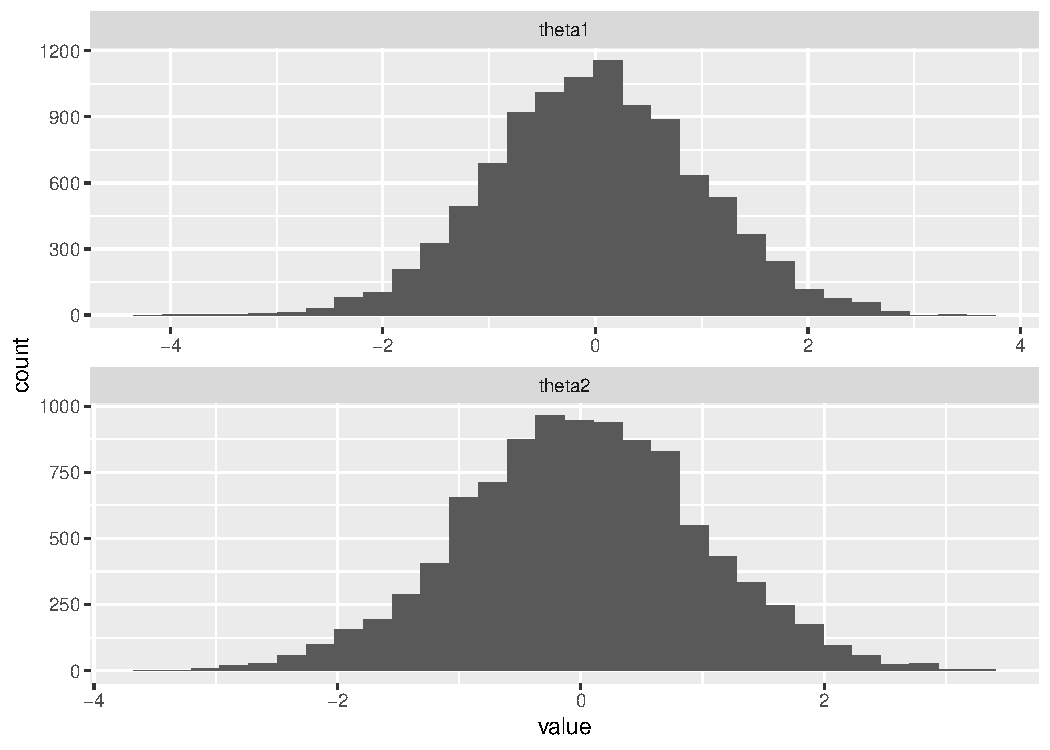
\includegraphics[width=0.8\linewidth]{Bayes_stat_hw3_files/figure-latex/unnamed-chunk-5-1} \end{center}

\begin{Shaded}
\begin{Highlighting}[]
\NormalTok{post\_1203 }\SpecialCharTok{\%\textgreater{}\%}\NormalTok{ mcmc }\SpecialCharTok{\%\textgreater{}\%}\NormalTok{ ggs }\SpecialCharTok{\%\textgreater{}\%} \FunctionTok{ggs\_density}\NormalTok{()}
\end{Highlighting}
\end{Shaded}

\begin{center}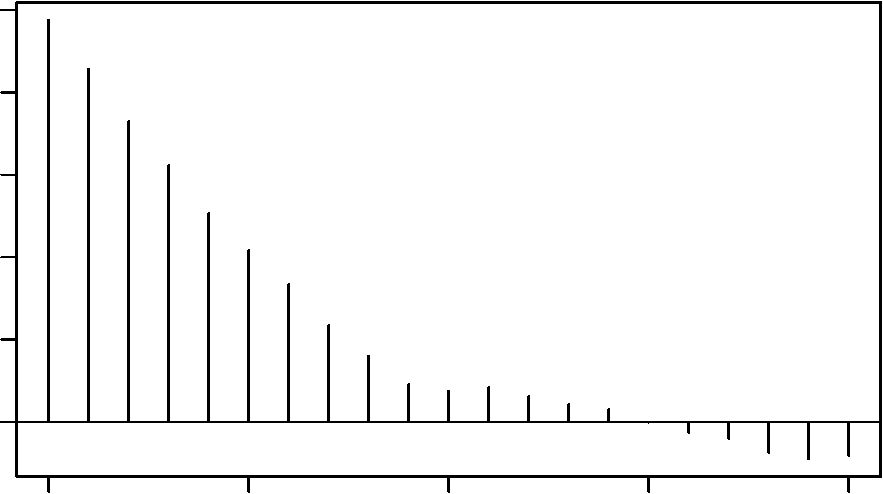
\includegraphics[width=0.8\linewidth]{Bayes_stat_hw3_files/figure-latex/unnamed-chunk-5-2} \end{center}

\paragraph{시계열 그림}\label{uxc2dcuxacc4uxc5f4-uxadf8uxb9bc}

\begin{Shaded}
\begin{Highlighting}[]
\NormalTok{post\_1203 }\SpecialCharTok{\%\textgreater{}\%}\NormalTok{ mcmc }\SpecialCharTok{\%\textgreater{}\%}\NormalTok{ ggs }\SpecialCharTok{\%\textgreater{}\%} \FunctionTok{ggs\_traceplot}\NormalTok{()}
\end{Highlighting}
\end{Shaded}

\begin{center}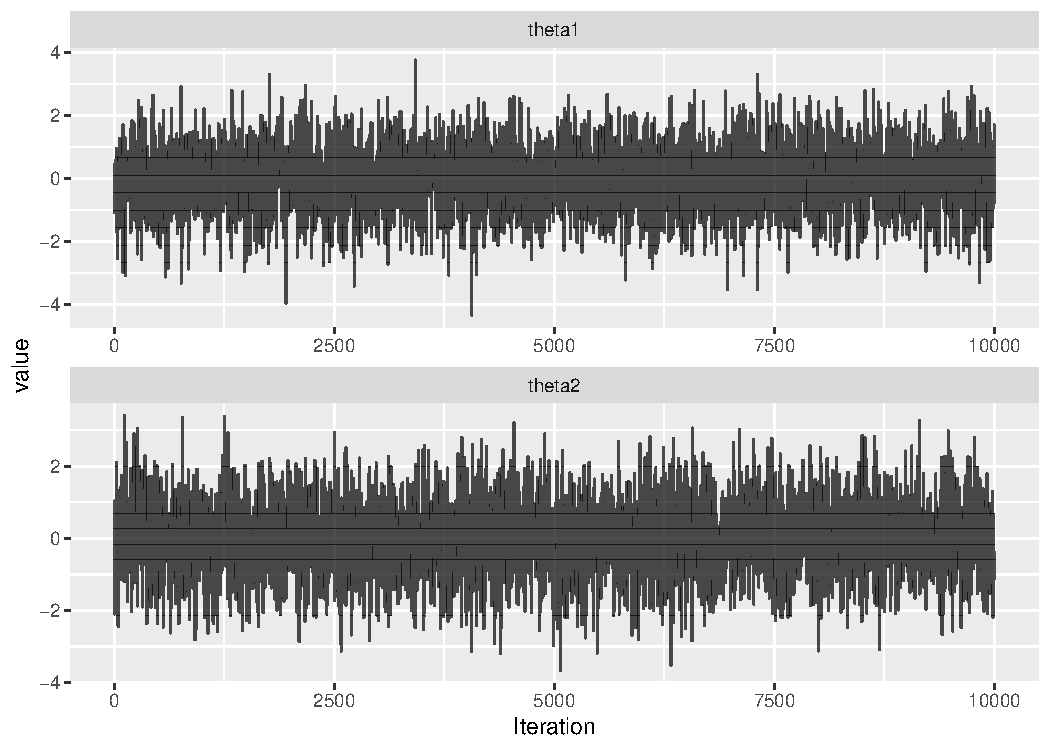
\includegraphics[width=0.8\linewidth]{Bayes_stat_hw3_files/figure-latex/unnamed-chunk-6-1} \end{center}

\paragraph{자기상관계수
그림}\label{uxc790uxae30uxc0c1uxad00uxacc4uxc218-uxadf8uxb9bc}

\begin{Shaded}
\begin{Highlighting}[]
\NormalTok{post\_1203 }\SpecialCharTok{\%\textgreater{}\%}\NormalTok{ mcmc }\SpecialCharTok{\%\textgreater{}\%}\NormalTok{ ggs }\SpecialCharTok{\%\textgreater{}\%} \FunctionTok{ggs\_autocorrelation}\NormalTok{()}
\end{Highlighting}
\end{Shaded}

\begin{center}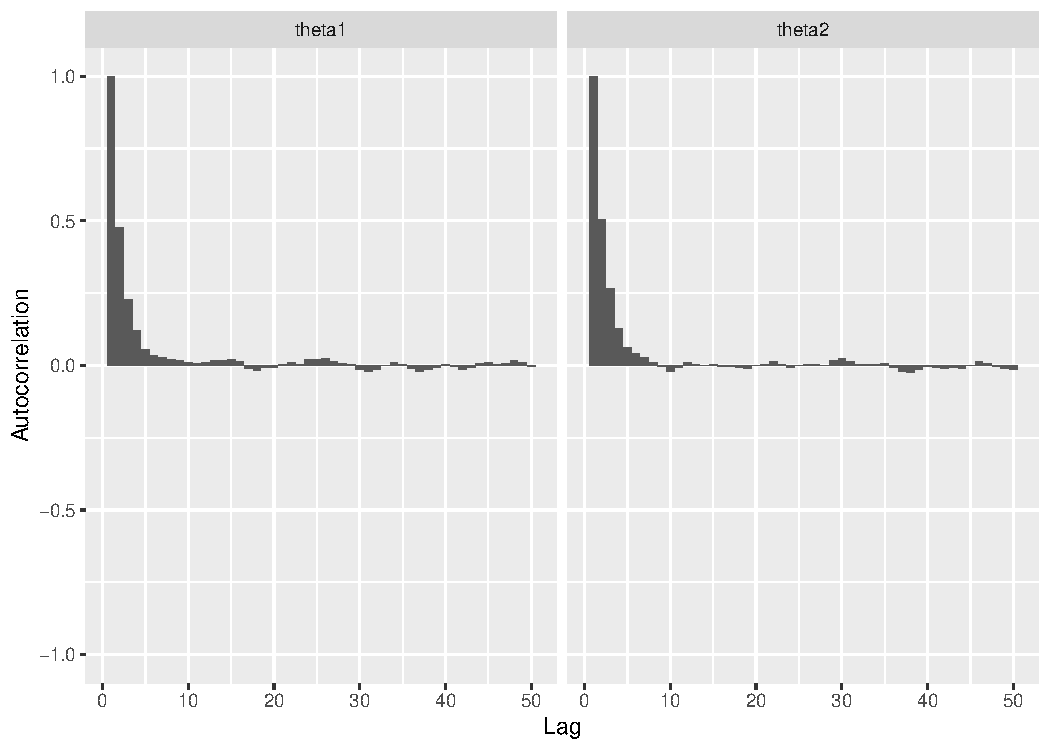
\includegraphics[width=0.8\linewidth]{Bayes_stat_hw3_files/figure-latex/unnamed-chunk-7-1} \end{center}

rho = 0.3에서는 시계열 그림이 특별한 경향을 보이지 않고, 자기상관계수
그림에서 확실히 자기상관계수가 감소하는 것으로 보아 마르코프 체인이
수렴하였다.

\subsubsection{사후표본 추출 - rho =
0.99}\label{uxc0acuxd6c4uxd45cuxbcf8-uxcd94uxcd9c---rho-0.99}

\begin{Shaded}
\begin{Highlighting}[]
\NormalTok{m }\OtherTok{=} \DecValTok{10000}
\NormalTok{rho }\OtherTok{=} \FloatTok{0.99}
\NormalTok{po.theta1 }\OtherTok{=} \ConstantTok{NULL}
\NormalTok{po.theta2 }\OtherTok{=} \ConstantTok{NULL}
\NormalTok{theta1 }\OtherTok{=} \DecValTok{0}
\NormalTok{theta2 }\OtherTok{=} \DecValTok{0}
\NormalTok{po.theta1 }\OtherTok{=} \FunctionTok{c}\NormalTok{(po.theta1, theta1)}
\NormalTok{po.theta2 }\OtherTok{=} \FunctionTok{c}\NormalTok{(po.theta2, theta2) }

\FunctionTok{set.seed}\NormalTok{(}\DecValTok{42}\NormalTok{) }\CommentTok{\#seed는 42로 고정.}
\ControlFlowTok{for}\NormalTok{ (i }\ControlFlowTok{in} \DecValTok{1}\SpecialCharTok{:}\NormalTok{m) \{ }\CommentTok{\#m = 10000회 동안 반복.}
\NormalTok{  proposal\_theta }\OtherTok{\textless{}{-}} \FunctionTok{rcauchy}\NormalTok{(}\DecValTok{2}\NormalTok{, }\AttributeTok{location =} \DecValTok{0}\NormalTok{, }\AttributeTok{scale =} \DecValTok{1}\NormalTok{) }\CommentTok{\#제안분포에서 난수 생성}
\NormalTok{  u }\OtherTok{\textless{}{-}} \FunctionTok{runif}\NormalTok{(}\DecValTok{1}\NormalTok{, }\AttributeTok{min =} \DecValTok{0}\NormalTok{, }\AttributeTok{max =} \DecValTok{1}\NormalTok{) }\CommentTok{\#합격{-}불합격 판정용 난수 생성}
\NormalTok{  accp\_prob }\OtherTok{\textless{}{-}} \FunctionTok{min}\NormalTok{(}\DecValTok{1}\NormalTok{,((}\DecValTok{1}\SpecialCharTok{+}\NormalTok{(proposal\_theta[}\DecValTok{1}\NormalTok{])}\SpecialCharTok{\^{}}\DecValTok{2}\NormalTok{)}\SpecialCharTok{*}\NormalTok{(}\DecValTok{1}\SpecialCharTok{+}\NormalTok{(proposal\_theta[}\DecValTok{2}\NormalTok{])}\SpecialCharTok{\^{}}\DecValTok{2}\NormalTok{)}\SpecialCharTok{*}\FunctionTok{exp}\NormalTok{(((po.theta1[i])}\SpecialCharTok{\^{}}\DecValTok{2}\SpecialCharTok{+}\NormalTok{(po.theta2[i])}\SpecialCharTok{\^{}}\DecValTok{2}\SpecialCharTok{{-}}\NormalTok{(proposal\_theta[}\DecValTok{1}\NormalTok{])}\SpecialCharTok{\^{}}\DecValTok{2}\SpecialCharTok{{-}}\NormalTok{(proposal\_theta[}\DecValTok{2}\NormalTok{])}\SpecialCharTok{\^{}}\DecValTok{2{-}2}\SpecialCharTok{*}\NormalTok{rho}\SpecialCharTok{*}\NormalTok{(po.theta1[i]}\SpecialCharTok{*}\NormalTok{po.theta2[i]}\SpecialCharTok{{-}}\NormalTok{proposal\_theta[}\DecValTok{1}\NormalTok{]}\SpecialCharTok{*}\NormalTok{proposal\_theta[}\DecValTok{2}\NormalTok{]))}\SpecialCharTok{/}\NormalTok{(}\DecValTok{2}\SpecialCharTok{*}\NormalTok{(}\DecValTok{1}\SpecialCharTok{{-}}\NormalTok{(rho)}\SpecialCharTok{\^{}}\DecValTok{2}\NormalTok{))))}\SpecialCharTok{/}\NormalTok{((}\DecValTok{1}\SpecialCharTok{+}\NormalTok{(po.theta1[i])}\SpecialCharTok{\^{}}\DecValTok{2}\NormalTok{)}\SpecialCharTok{*}\NormalTok{(}\DecValTok{1}\SpecialCharTok{+}\NormalTok{(po.theta2[i])}\SpecialCharTok{\^{}}\DecValTok{2}\NormalTok{)))}
  \ControlFlowTok{if}\NormalTok{(accp\_prob }\SpecialCharTok{\textgreater{}=}\NormalTok{ u)\{}
\NormalTok{    po.theta1 }\OtherTok{\textless{}{-}} \FunctionTok{c}\NormalTok{(po.theta1, proposal\_theta[}\DecValTok{1}\NormalTok{])}
\NormalTok{    po.theta2 }\OtherTok{\textless{}{-}} \FunctionTok{c}\NormalTok{(po.theta2, proposal\_theta[}\DecValTok{2}\NormalTok{])}
\NormalTok{  \} }\ControlFlowTok{else}\NormalTok{\{}
\NormalTok{    po.theta1 }\OtherTok{\textless{}{-}} \FunctionTok{c}\NormalTok{(po.theta1, po.theta1[i])}
\NormalTok{    po.theta2 }\OtherTok{\textless{}{-}} \FunctionTok{c}\NormalTok{(po.theta2, po.theta2[i])}
\NormalTok{  \}}
\NormalTok{\}}

\NormalTok{post\_1299 }\OtherTok{\textless{}{-}} \FunctionTok{data.frame}\NormalTok{(}\AttributeTok{theta1 =}\NormalTok{ po.theta1, }\AttributeTok{theta2 =}\NormalTok{ po.theta2)}
\end{Highlighting}
\end{Shaded}

\paragraph{히스토그램}\label{uxd788uxc2a4uxd1a0uxadf8uxb7a8-1}

\begin{Shaded}
\begin{Highlighting}[]
\NormalTok{post\_1299 }\SpecialCharTok{\%\textgreater{}\%}\NormalTok{ mcmc }\SpecialCharTok{\%\textgreater{}\%}\NormalTok{ ggs }\SpecialCharTok{\%\textgreater{}\%} \FunctionTok{ggs\_histogram}\NormalTok{()}
\end{Highlighting}
\end{Shaded}

\begin{center}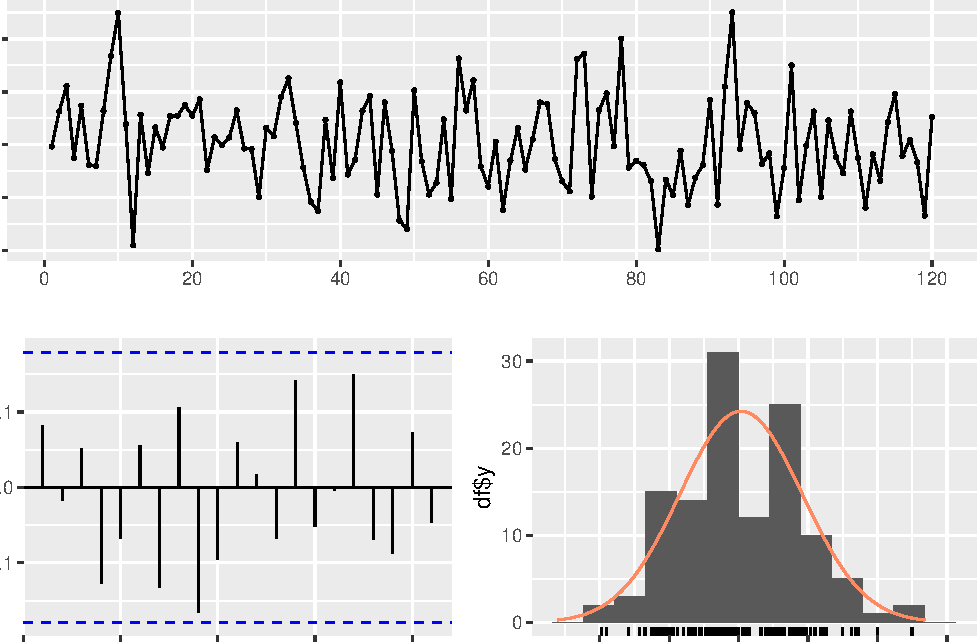
\includegraphics[width=0.8\linewidth]{Bayes_stat_hw3_files/figure-latex/unnamed-chunk-9-1} \end{center}

\begin{Shaded}
\begin{Highlighting}[]
\NormalTok{post\_1299 }\SpecialCharTok{\%\textgreater{}\%}\NormalTok{ mcmc }\SpecialCharTok{\%\textgreater{}\%}\NormalTok{ ggs }\SpecialCharTok{\%\textgreater{}\%} \FunctionTok{ggs\_density}\NormalTok{()}
\end{Highlighting}
\end{Shaded}

\begin{center}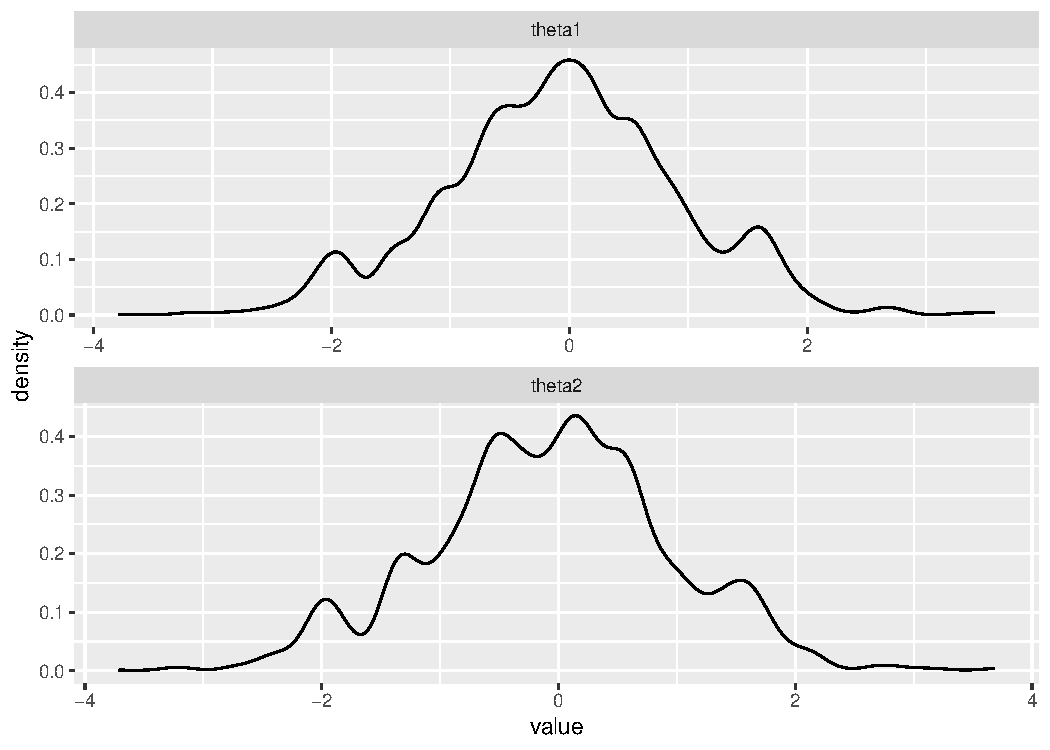
\includegraphics[width=0.8\linewidth]{Bayes_stat_hw3_files/figure-latex/unnamed-chunk-9-2} \end{center}

\paragraph{시계열 그림}\label{uxc2dcuxacc4uxc5f4-uxadf8uxb9bc-1}

\begin{Shaded}
\begin{Highlighting}[]
\NormalTok{post\_1299 }\SpecialCharTok{\%\textgreater{}\%}\NormalTok{ mcmc }\SpecialCharTok{\%\textgreater{}\%}\NormalTok{ ggs }\SpecialCharTok{\%\textgreater{}\%} \FunctionTok{ggs\_traceplot}\NormalTok{()}
\end{Highlighting}
\end{Shaded}

\begin{center}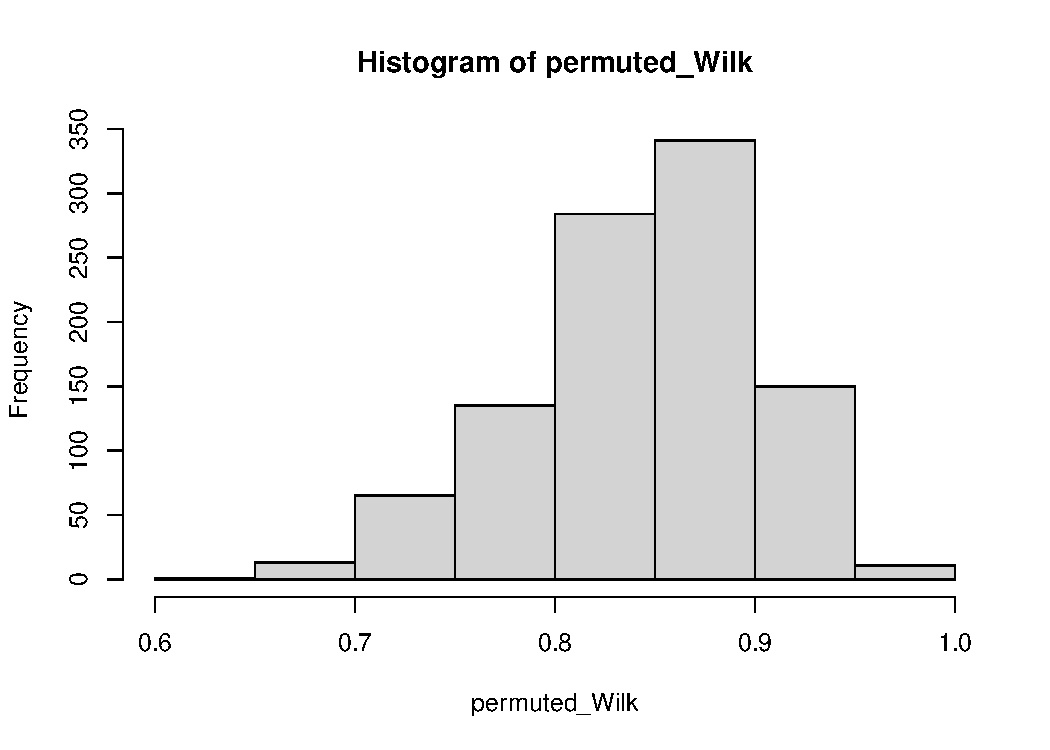
\includegraphics[width=0.8\linewidth]{Bayes_stat_hw3_files/figure-latex/unnamed-chunk-10-1} \end{center}

\paragraph{자기상관계수
그림}\label{uxc790uxae30uxc0c1uxad00uxacc4uxc218-uxadf8uxb9bc-1}

\begin{Shaded}
\begin{Highlighting}[]
\NormalTok{post\_1299 }\SpecialCharTok{\%\textgreater{}\%}\NormalTok{ mcmc }\SpecialCharTok{\%\textgreater{}\%}\NormalTok{ ggs }\SpecialCharTok{\%\textgreater{}\%} \FunctionTok{ggs\_autocorrelation}\NormalTok{()}
\end{Highlighting}
\end{Shaded}

\begin{center}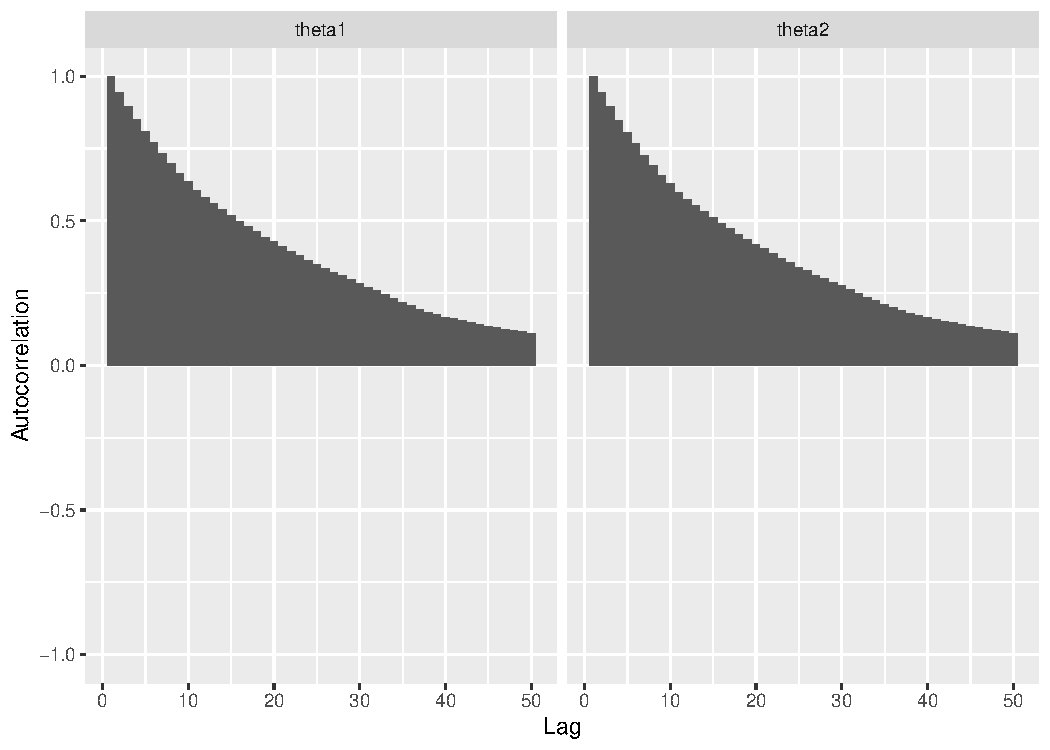
\includegraphics[width=0.8\linewidth]{Bayes_stat_hw3_files/figure-latex/unnamed-chunk-11-1} \end{center}

rho = 0.99에서는 히스토그램이 정규분포의 모양이 아니고, 자기상관계수
그림에서 자기상관계수가 느리게 감소하고, 시계열 그림에서 아직 특정한
경향이 보이는 등 마르코프 체인이 수렴하지 않았다. 이 경우 m이 부족하므로
표본의 수를 늘려야 한다.

\subsection{(d)}\label{d}

\subsubsection{\texorpdfstring{\(\rho\) =
0.3}{\textbackslash rho = 0.3}}\label{rho-0.3}

\begin{Shaded}
\begin{Highlighting}[]
\NormalTok{post\_1203 }\SpecialCharTok{\%\textgreater{}\%}\NormalTok{ mcmc }\SpecialCharTok{\%\textgreater{}\%}\NormalTok{ summary}
\end{Highlighting}
\end{Shaded}

\begin{verbatim}
## 
## Iterations = 1:10001
## Thinning interval = 1 
## Number of chains = 1 
## Sample size per chain = 10001 
## 
## 1. Empirical mean and standard deviation for each variable,
##    plus standard error of the mean:
## 
##             Mean     SD Naive SE Time-series SE
## theta1 -0.005994 0.9758 0.009758        0.01641
## theta2  0.003006 0.9766 0.009766        0.01706
## 
## 2. Quantiles for each variable:
## 
##          2.5%     25%       50%    75% 97.5%
## theta1 -1.882 -0.6763 -0.007666 0.6252 1.913
## theta2 -1.946 -0.6400  0.006172 0.6391 1.930
\end{verbatim}

\begin{verbatim}
     2.5%     25%       50%    75% 97.5%    Mean     SD
\end{verbatim}

theta1 -1.882 -0.6763 -0.007666 0.6252 1.913 -0.005994 0.9758 theta2
-1.946 -0.6400 0.006172 0.6391 1.930 0.003006 0.9766

\subsubsection{\texorpdfstring{\(\rho\) =
0.99}{\textbackslash rho = 0.99}}\label{rho-0.99}

\begin{Shaded}
\begin{Highlighting}[]
\NormalTok{post\_1299 }\SpecialCharTok{\%\textgreater{}\%}\NormalTok{ mcmc }\SpecialCharTok{\%\textgreater{}\%}\NormalTok{ summary}
\end{Highlighting}
\end{Shaded}

\begin{verbatim}
## 
## Iterations = 1:10001
## Thinning interval = 1 
## Number of chains = 1 
## Sample size per chain = 10001 
## 
## 1. Empirical mean and standard deviation for each variable,
##    plus standard error of the mean:
## 
##            Mean     SD Naive SE Time-series SE
## theta1 -0.06298 0.9914 0.009914        0.06733
## theta2 -0.06421 1.0126 0.010126        0.06817
## 
## 2. Quantiles for each variable:
## 
##          2.5%     25%      50%    75% 97.5%
## theta1 -2.032 -0.6890 -0.05691 0.5526 1.772
## theta2 -2.052 -0.6667 -0.03836 0.5900 1.801
\end{verbatim}

\begin{verbatim}
     2.5%     25%      50%    75% 97.5%   Mean     SD
\end{verbatim}

theta1 -2.032 -0.6890 -0.05691 0.5526 1.772 -0.06298 0.9914 theta2
-2.052 -0.6667 -0.03836 0.5900 1.801 -0.06421 1.0126

\section{1.9.13}\label{section-1}

\subsection{(a)}\label{a-1}

해당 문제는 종이에 풀이하였다.

\subsection{(b)}\label{b-1}

\subsubsection{초기화}\label{uxcd08uxae30uxd654-1}

\begin{Shaded}
\begin{Highlighting}[]
\NormalTok{m }\OtherTok{=} \DecValTok{5000}
\NormalTok{rho }\OtherTok{=} \FloatTok{0.99}
\NormalTok{cov\_mtx }\OtherTok{\textless{}{-}} \FunctionTok{matrix}\NormalTok{(}\FunctionTok{c}\NormalTok{(}\DecValTok{1}\NormalTok{, rho, rho, }\DecValTok{1}\NormalTok{), }\AttributeTok{nrow =} \DecValTok{2}\NormalTok{)}
\NormalTok{d }\OtherTok{=} \DecValTok{1} \CommentTok{\#d는 적절한 합격률이 되도록 해야 함. }
\NormalTok{po.theta1 }\OtherTok{=} \ConstantTok{NULL}
\NormalTok{po.theta2 }\OtherTok{=} \ConstantTok{NULL}
\NormalTok{theta1 }\OtherTok{=} \DecValTok{0}
\NormalTok{theta2 }\OtherTok{=} \DecValTok{0}
\NormalTok{po.theta1 }\OtherTok{=} \FunctionTok{c}\NormalTok{(po.theta1, theta1)}
\NormalTok{po.theta2 }\OtherTok{=} \FunctionTok{c}\NormalTok{(po.theta2, theta2) }
\end{Highlighting}
\end{Shaded}

우선, theta1 = theta2 = 0으로 초기화하였다. 이 문제에서는 우선 m = 5000,
rho = 0.99로 두었다.

\subsubsection{메트로폴리스-헤이스팅스
반복}\label{uxba54uxd2b8uxb85cuxd3f4uxb9acuxc2a4-uxd5e4uxc774uxc2a4uxd305uxc2a4-uxbc18uxbcf5-1}

\begin{Shaded}
\begin{Highlighting}[]
\FunctionTok{set.seed}\NormalTok{(}\DecValTok{42}\NormalTok{) }
\ControlFlowTok{for}\NormalTok{ (i }\ControlFlowTok{in} \DecValTok{1}\SpecialCharTok{:}\NormalTok{m) \{}\CommentTok{\#m = 5000회 동안 반복.}
\NormalTok{  proposal\_theta1 }\OtherTok{\textless{}{-}} \FunctionTok{rnorm}\NormalTok{(}\DecValTok{1}\NormalTok{, po.theta1[i], d)}
\NormalTok{  proposal\_theta2 }\OtherTok{\textless{}{-}} \FunctionTok{rcauchy}\NormalTok{(}\DecValTok{1}\NormalTok{, }\AttributeTok{location =} \DecValTok{0}\NormalTok{, }\AttributeTok{scale =} \DecValTok{1}\NormalTok{) }\CommentTok{\#제안분포에서 난수 생성}
\NormalTok{  u }\OtherTok{\textless{}{-}} \FunctionTok{runif}\NormalTok{(}\DecValTok{1}\NormalTok{, }\AttributeTok{min =} \DecValTok{0}\NormalTok{, }\AttributeTok{max =} \DecValTok{1}\NormalTok{) }\CommentTok{\#합격{-}불합격 판정용 난수 생성}
\NormalTok{  accp\_prob }\OtherTok{\textless{}{-}} \FunctionTok{min}\NormalTok{(}\DecValTok{1}\NormalTok{, (}\FunctionTok{dmvnorm}\NormalTok{(}\FunctionTok{c}\NormalTok{(proposal\_theta1, proposal\_theta2), }\FunctionTok{c}\NormalTok{(}\DecValTok{0}\NormalTok{, }\DecValTok{0}\NormalTok{), cov\_mtx)}\SpecialCharTok{*}\FunctionTok{dcauchy}\NormalTok{(po.theta2[i], }\DecValTok{0}\NormalTok{, }\DecValTok{1}\NormalTok{))}\SpecialCharTok{/}\NormalTok{(}\FunctionTok{dmvnorm}\NormalTok{(}\FunctionTok{c}\NormalTok{(po.theta1[i], po.theta2[i]), }\FunctionTok{c}\NormalTok{(}\DecValTok{0}\NormalTok{, }\DecValTok{0}\NormalTok{), cov\_mtx)}\SpecialCharTok{*}\FunctionTok{dcauchy}\NormalTok{(proposal\_theta2, }\DecValTok{0}\NormalTok{, }\DecValTok{1}\NormalTok{)))}
  \ControlFlowTok{if}\NormalTok{(accp\_prob }\SpecialCharTok{\textgreater{}=}\NormalTok{ u)\{}
\NormalTok{    po.theta1 }\OtherTok{\textless{}{-}} \FunctionTok{c}\NormalTok{(po.theta1, proposal\_theta1)}
\NormalTok{    po.theta2 }\OtherTok{\textless{}{-}} \FunctionTok{c}\NormalTok{(po.theta2, proposal\_theta2)}
\NormalTok{  \} }\ControlFlowTok{else}\NormalTok{\{}
\NormalTok{    po.theta1 }\OtherTok{\textless{}{-}} \FunctionTok{c}\NormalTok{(po.theta1, po.theta1[i])}
\NormalTok{    po.theta2 }\OtherTok{\textless{}{-}} \FunctionTok{c}\NormalTok{(po.theta2, po.theta2[i])}
\NormalTok{  \}}
\NormalTok{\}}
\end{Highlighting}
\end{Shaded}

\subsubsection{확률변수
확인}\label{uxd655uxb960uxbcc0uxc218-uxd655uxc778-1}

\begin{Shaded}
\begin{Highlighting}[]
\FunctionTok{head}\NormalTok{(po.theta1)}
\end{Highlighting}
\end{Shaded}

\begin{verbatim}
## [1] 0 0 0 0 0 0
\end{verbatim}

\begin{Shaded}
\begin{Highlighting}[]
\FunctionTok{head}\NormalTok{(po.theta2)}
\end{Highlighting}
\end{Shaded}

\begin{verbatim}
## [1] 0 0 0 0 0 0
\end{verbatim}

이와 같이 추출된 po.theta1과 po.theta2는 이변량정규분포를 불변분포로
갖는 마르코프 체인이다.

\subsection{(c)}\label{c-1}

사후분포를 생성하기 전, 시범적인 난수 생성을 통해 \texttt{d}의 값을
결정해야 한다. seed를 지금까지 써 왔던 42가 아니라 31로 써서, \(\rho\) =
0.99와 0.3 각각에 대해 적절한 d 값을 찾아보겠다.

\begin{Shaded}
\begin{Highlighting}[]
\NormalTok{m }\OtherTok{=} \DecValTok{500}
\NormalTok{rho }\OtherTok{=} \FloatTok{0.99}
\NormalTok{cov\_mtx }\OtherTok{\textless{}{-}} \FunctionTok{matrix}\NormalTok{(}\FunctionTok{c}\NormalTok{(}\DecValTok{1}\NormalTok{, rho, rho, }\DecValTok{1}\NormalTok{), }\AttributeTok{nrow =} \DecValTok{2}\NormalTok{)}
\NormalTok{d }\OtherTok{=} \FloatTok{0.1} \CommentTok{\#d는 적절한 합격률이 되도록 해야 함. }
\NormalTok{accepted }\OtherTok{=} \DecValTok{0}
\NormalTok{po.theta1 }\OtherTok{=} \ConstantTok{NULL}
\NormalTok{po.theta2 }\OtherTok{=} \ConstantTok{NULL}
\NormalTok{theta1 }\OtherTok{=} \DecValTok{0}
\NormalTok{theta2 }\OtherTok{=} \DecValTok{0}
\NormalTok{po.theta1 }\OtherTok{=} \FunctionTok{c}\NormalTok{(po.theta1, theta1)}
\NormalTok{po.theta2 }\OtherTok{=} \FunctionTok{c}\NormalTok{(po.theta2, theta2) }

\FunctionTok{set.seed}\NormalTok{(}\DecValTok{31}\NormalTok{)}
\ControlFlowTok{for}\NormalTok{ (i }\ControlFlowTok{in} \DecValTok{1}\SpecialCharTok{:}\NormalTok{m) \{}\CommentTok{\#m = 5000회 동안 반복.}
\NormalTok{  proposal\_theta1 }\OtherTok{\textless{}{-}} \FunctionTok{rnorm}\NormalTok{(}\DecValTok{1}\NormalTok{, po.theta1[i], d)}
\NormalTok{  proposal\_theta2 }\OtherTok{\textless{}{-}} \FunctionTok{rcauchy}\NormalTok{(}\DecValTok{1}\NormalTok{, }\AttributeTok{location =} \DecValTok{0}\NormalTok{, }\AttributeTok{scale =} \DecValTok{1}\NormalTok{) }\CommentTok{\#제안분포에서 난수 생성}
\NormalTok{  u }\OtherTok{\textless{}{-}} \FunctionTok{runif}\NormalTok{(}\DecValTok{1}\NormalTok{, }\AttributeTok{min =} \DecValTok{0}\NormalTok{, }\AttributeTok{max =} \DecValTok{1}\NormalTok{) }\CommentTok{\#합격{-}불합격 판정용 난수 생성}
\NormalTok{  accp\_prob }\OtherTok{\textless{}{-}} \FunctionTok{min}\NormalTok{(}\DecValTok{1}\NormalTok{, (}\FunctionTok{dmvnorm}\NormalTok{(}\FunctionTok{c}\NormalTok{(proposal\_theta1, proposal\_theta2), }\FunctionTok{c}\NormalTok{(}\DecValTok{0}\NormalTok{, }\DecValTok{0}\NormalTok{), cov\_mtx)}\SpecialCharTok{*}\FunctionTok{dcauchy}\NormalTok{(po.theta2[i], }\DecValTok{0}\NormalTok{, }\DecValTok{1}\NormalTok{))}\SpecialCharTok{/}\NormalTok{(}\FunctionTok{dmvnorm}\NormalTok{(}\FunctionTok{c}\NormalTok{(po.theta1[i], po.theta2[i]), }\FunctionTok{c}\NormalTok{(}\DecValTok{0}\NormalTok{, }\DecValTok{0}\NormalTok{), cov\_mtx)}\SpecialCharTok{*}\FunctionTok{dcauchy}\NormalTok{(proposal\_theta2, }\DecValTok{0}\NormalTok{, }\DecValTok{1}\NormalTok{)))}
  \ControlFlowTok{if}\NormalTok{(accp\_prob }\SpecialCharTok{\textgreater{}=}\NormalTok{ u)\{}
\NormalTok{    accepted }\OtherTok{\textless{}{-}}\NormalTok{ accepted }\SpecialCharTok{+} \DecValTok{1}
\NormalTok{    po.theta1 }\OtherTok{\textless{}{-}} \FunctionTok{c}\NormalTok{(po.theta1, proposal\_theta1)}
\NormalTok{    po.theta2 }\OtherTok{\textless{}{-}} \FunctionTok{c}\NormalTok{(po.theta2, proposal\_theta2)}
\NormalTok{  \} }\ControlFlowTok{else}\NormalTok{\{}
\NormalTok{    po.theta1 }\OtherTok{\textless{}{-}} \FunctionTok{c}\NormalTok{(po.theta1, po.theta1[i])}
\NormalTok{    po.theta2 }\OtherTok{\textless{}{-}} \FunctionTok{c}\NormalTok{(po.theta2, po.theta2[i])}
\NormalTok{  \}}
\NormalTok{\}}

\NormalTok{accepted}\SpecialCharTok{/}\DecValTok{500}
\end{Highlighting}
\end{Shaded}

\begin{verbatim}
## [1] 0.12
\end{verbatim}

\(\rho\) = 0.99 케이스에서는 d값이 지나치게 작아지는 것이 바람직하지
않아 보여 0.25를 달성하지 못하고 성능 개선이 낮은 수준인 0.1 수준에서
중단하였다.

\begin{Shaded}
\begin{Highlighting}[]
\NormalTok{m }\OtherTok{=} \DecValTok{500}
\NormalTok{rho }\OtherTok{=} \FloatTok{0.3}
\NormalTok{cov\_mtx }\OtherTok{\textless{}{-}} \FunctionTok{matrix}\NormalTok{(}\FunctionTok{c}\NormalTok{(}\DecValTok{1}\NormalTok{, rho, rho, }\DecValTok{1}\NormalTok{), }\AttributeTok{nrow =} \DecValTok{2}\NormalTok{)}
\NormalTok{d }\OtherTok{=} \DecValTok{3} \CommentTok{\#d는 적절한 합격률이 되도록 해야 함. }
\NormalTok{accepted }\OtherTok{=} \DecValTok{0}
\NormalTok{po.theta1 }\OtherTok{=} \ConstantTok{NULL}
\NormalTok{po.theta2 }\OtherTok{=} \ConstantTok{NULL}
\NormalTok{theta1 }\OtherTok{=} \DecValTok{0}
\NormalTok{theta2 }\OtherTok{=} \DecValTok{0}
\NormalTok{po.theta1 }\OtherTok{=} \FunctionTok{c}\NormalTok{(po.theta1, theta1)}
\NormalTok{po.theta2 }\OtherTok{=} \FunctionTok{c}\NormalTok{(po.theta2, theta2) }

\FunctionTok{set.seed}\NormalTok{(}\DecValTok{31}\NormalTok{)}
\ControlFlowTok{for}\NormalTok{ (i }\ControlFlowTok{in} \DecValTok{1}\SpecialCharTok{:}\NormalTok{m) \{}\CommentTok{\#m = 5000회 동안 반복.}
\NormalTok{  proposal\_theta1 }\OtherTok{\textless{}{-}} \FunctionTok{rnorm}\NormalTok{(}\DecValTok{1}\NormalTok{, po.theta1[i], d)}
\NormalTok{  proposal\_theta2 }\OtherTok{\textless{}{-}} \FunctionTok{rcauchy}\NormalTok{(}\DecValTok{1}\NormalTok{, }\AttributeTok{location =} \DecValTok{0}\NormalTok{, }\AttributeTok{scale =} \DecValTok{1}\NormalTok{) }\CommentTok{\#제안분포에서 난수 생성}
\NormalTok{  u }\OtherTok{\textless{}{-}} \FunctionTok{runif}\NormalTok{(}\DecValTok{1}\NormalTok{, }\AttributeTok{min =} \DecValTok{0}\NormalTok{, }\AttributeTok{max =} \DecValTok{1}\NormalTok{) }\CommentTok{\#합격{-}불합격 판정용 난수 생성}
\NormalTok{  accp\_prob }\OtherTok{\textless{}{-}} \FunctionTok{min}\NormalTok{(}\DecValTok{1}\NormalTok{, (}\FunctionTok{dmvnorm}\NormalTok{(}\FunctionTok{c}\NormalTok{(proposal\_theta1, proposal\_theta2), }\FunctionTok{c}\NormalTok{(}\DecValTok{0}\NormalTok{, }\DecValTok{0}\NormalTok{), cov\_mtx)}\SpecialCharTok{*}\FunctionTok{dcauchy}\NormalTok{(po.theta2[i], }\DecValTok{0}\NormalTok{, }\DecValTok{1}\NormalTok{))}\SpecialCharTok{/}\NormalTok{(}\FunctionTok{dmvnorm}\NormalTok{(}\FunctionTok{c}\NormalTok{(po.theta1[i], po.theta2[i]), }\FunctionTok{c}\NormalTok{(}\DecValTok{0}\NormalTok{, }\DecValTok{0}\NormalTok{), cov\_mtx)}\SpecialCharTok{*}\FunctionTok{dcauchy}\NormalTok{(proposal\_theta2, }\DecValTok{0}\NormalTok{, }\DecValTok{1}\NormalTok{)))}
  \ControlFlowTok{if}\NormalTok{(accp\_prob }\SpecialCharTok{\textgreater{}=}\NormalTok{ u)\{}
\NormalTok{    accepted }\OtherTok{\textless{}{-}}\NormalTok{ accepted }\SpecialCharTok{+} \DecValTok{1}
\NormalTok{    po.theta1 }\OtherTok{\textless{}{-}} \FunctionTok{c}\NormalTok{(po.theta1, proposal\_theta1)}
\NormalTok{    po.theta2 }\OtherTok{\textless{}{-}} \FunctionTok{c}\NormalTok{(po.theta2, proposal\_theta2)}
\NormalTok{  \} }\ControlFlowTok{else}\NormalTok{\{}
\NormalTok{    po.theta1 }\OtherTok{\textless{}{-}} \FunctionTok{c}\NormalTok{(po.theta1, po.theta1[i])}
\NormalTok{    po.theta2 }\OtherTok{\textless{}{-}} \FunctionTok{c}\NormalTok{(po.theta2, po.theta2[i])}
\NormalTok{  \}}
\NormalTok{\}}

\NormalTok{accepted}\SpecialCharTok{/}\DecValTok{500}
\end{Highlighting}
\end{Shaded}

\begin{verbatim}
## [1] 0.244
\end{verbatim}

\(\rho\) = 0.3 케이스에서는 d = 3 수준이 적절한 합격률을 보였다. 이제 이
값을 바탕으로 각각 5000개 사후표본을 생성한다.

\subsubsection{\texorpdfstring{\(\rho\) =
0.99}{\textbackslash rho = 0.99}}\label{rho-0.99-1}

\begin{Shaded}
\begin{Highlighting}[]
\NormalTok{m }\OtherTok{=} \DecValTok{5000}
\NormalTok{rho }\OtherTok{=} \FloatTok{0.99}
\NormalTok{cov\_mtx }\OtherTok{\textless{}{-}} \FunctionTok{matrix}\NormalTok{(}\FunctionTok{c}\NormalTok{(}\DecValTok{1}\NormalTok{, rho, rho, }\DecValTok{1}\NormalTok{), }\AttributeTok{nrow =} \DecValTok{2}\NormalTok{)}
\NormalTok{d }\OtherTok{=} \FloatTok{0.1}
\NormalTok{po.theta1 }\OtherTok{=} \ConstantTok{NULL}
\NormalTok{po.theta2 }\OtherTok{=} \ConstantTok{NULL}
\NormalTok{theta1 }\OtherTok{=} \DecValTok{0}
\NormalTok{theta2 }\OtherTok{=} \DecValTok{0}
\NormalTok{po.theta1 }\OtherTok{=} \FunctionTok{c}\NormalTok{(po.theta1, theta1)}
\NormalTok{po.theta2 }\OtherTok{=} \FunctionTok{c}\NormalTok{(po.theta2, theta2) }

\FunctionTok{set.seed}\NormalTok{(}\DecValTok{42}\NormalTok{)}
\ControlFlowTok{for}\NormalTok{ (i }\ControlFlowTok{in} \DecValTok{1}\SpecialCharTok{:}\NormalTok{m) \{}\CommentTok{\#m = 5000회 동안 반복.}
\NormalTok{  proposal\_theta1 }\OtherTok{\textless{}{-}} \FunctionTok{rnorm}\NormalTok{(}\DecValTok{1}\NormalTok{, po.theta1[i], d)}
\NormalTok{  proposal\_theta2 }\OtherTok{\textless{}{-}} \FunctionTok{rcauchy}\NormalTok{(}\DecValTok{1}\NormalTok{, }\AttributeTok{location =} \DecValTok{0}\NormalTok{, }\AttributeTok{scale =} \DecValTok{1}\NormalTok{) }\CommentTok{\#제안분포에서 난수 생성}
\NormalTok{  u }\OtherTok{\textless{}{-}} \FunctionTok{runif}\NormalTok{(}\DecValTok{1}\NormalTok{, }\AttributeTok{min =} \DecValTok{0}\NormalTok{, }\AttributeTok{max =} \DecValTok{1}\NormalTok{) }\CommentTok{\#합격{-}불합격 판정용 난수 생성}
\NormalTok{  accp\_prob }\OtherTok{\textless{}{-}} \FunctionTok{min}\NormalTok{(}\DecValTok{1}\NormalTok{, (}\FunctionTok{dmvnorm}\NormalTok{(}\FunctionTok{c}\NormalTok{(proposal\_theta1, proposal\_theta2), }\FunctionTok{c}\NormalTok{(}\DecValTok{0}\NormalTok{, }\DecValTok{0}\NormalTok{), cov\_mtx)}\SpecialCharTok{*}\FunctionTok{dcauchy}\NormalTok{(po.theta2[i], }\DecValTok{0}\NormalTok{, }\DecValTok{1}\NormalTok{))}\SpecialCharTok{/}\NormalTok{(}\FunctionTok{dmvnorm}\NormalTok{(}\FunctionTok{c}\NormalTok{(po.theta1[i], po.theta2[i]), }\FunctionTok{c}\NormalTok{(}\DecValTok{0}\NormalTok{, }\DecValTok{0}\NormalTok{), cov\_mtx)}\SpecialCharTok{*}\FunctionTok{dcauchy}\NormalTok{(proposal\_theta2, }\DecValTok{0}\NormalTok{, }\DecValTok{1}\NormalTok{)))}
  \ControlFlowTok{if}\NormalTok{(accp\_prob }\SpecialCharTok{\textgreater{}=}\NormalTok{ u)\{}
\NormalTok{    po.theta1 }\OtherTok{\textless{}{-}} \FunctionTok{c}\NormalTok{(po.theta1, proposal\_theta1)}
\NormalTok{    po.theta2 }\OtherTok{\textless{}{-}} \FunctionTok{c}\NormalTok{(po.theta2, proposal\_theta2)}
\NormalTok{  \} }\ControlFlowTok{else}\NormalTok{\{}
\NormalTok{    po.theta1 }\OtherTok{\textless{}{-}} \FunctionTok{c}\NormalTok{(po.theta1, po.theta1[i])}
\NormalTok{    po.theta2 }\OtherTok{\textless{}{-}} \FunctionTok{c}\NormalTok{(po.theta2, po.theta2[i])}
\NormalTok{  \}}
\NormalTok{\}}

\NormalTok{post\_1399 }\OtherTok{\textless{}{-}} \FunctionTok{data.frame}\NormalTok{(}\AttributeTok{theta1 =}\NormalTok{ po.theta1, }\AttributeTok{theta2 =}\NormalTok{ po.theta2)}
\end{Highlighting}
\end{Shaded}

\paragraph{히스토그램}\label{uxd788uxc2a4uxd1a0uxadf8uxb7a8-2}

\begin{Shaded}
\begin{Highlighting}[]
\NormalTok{post\_1399 }\SpecialCharTok{\%\textgreater{}\%}\NormalTok{ mcmc }\SpecialCharTok{\%\textgreater{}\%}\NormalTok{ ggs }\SpecialCharTok{\%\textgreater{}\%} \FunctionTok{ggs\_histogram}\NormalTok{()}
\end{Highlighting}
\end{Shaded}

\begin{center}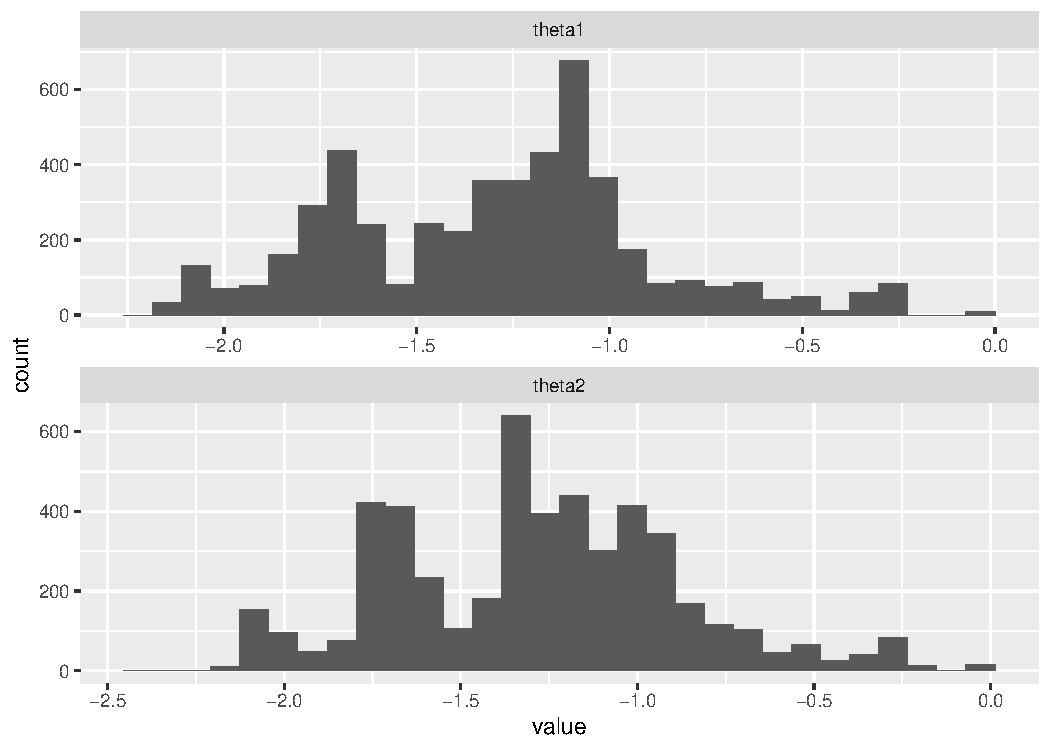
\includegraphics[width=0.8\linewidth]{Bayes_stat_hw3_files/figure-latex/unnamed-chunk-20-1} \end{center}

\begin{Shaded}
\begin{Highlighting}[]
\NormalTok{post\_1399 }\SpecialCharTok{\%\textgreater{}\%}\NormalTok{ mcmc }\SpecialCharTok{\%\textgreater{}\%}\NormalTok{ ggs }\SpecialCharTok{\%\textgreater{}\%} \FunctionTok{ggs\_density}\NormalTok{()}
\end{Highlighting}
\end{Shaded}

\begin{center}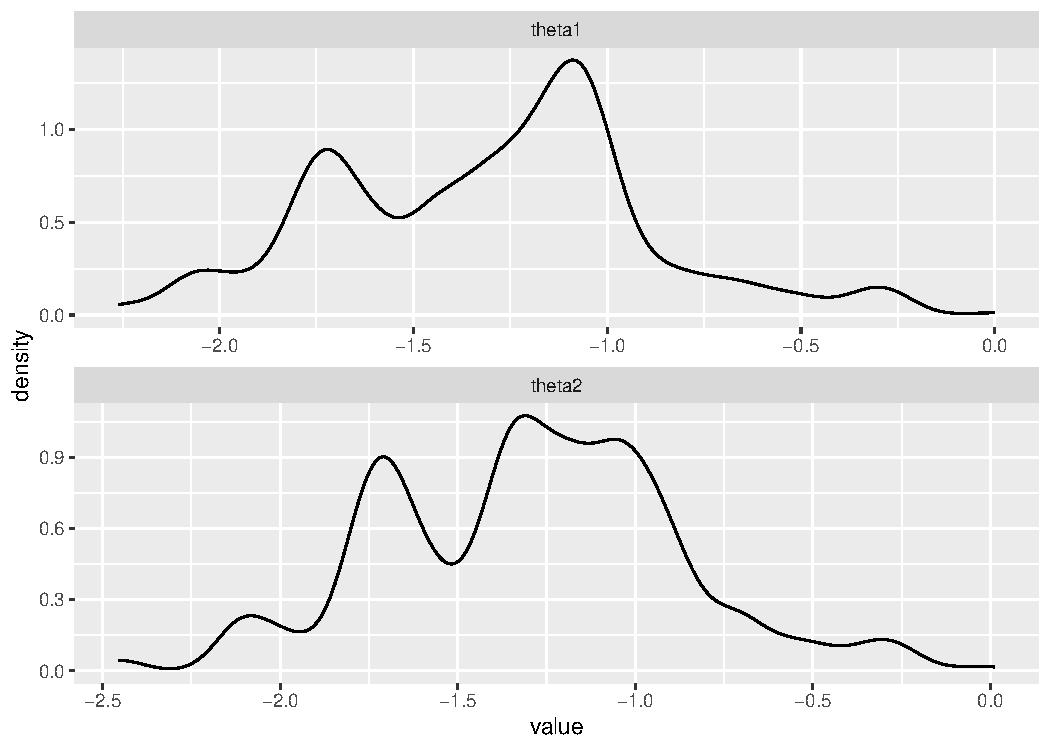
\includegraphics[width=0.8\linewidth]{Bayes_stat_hw3_files/figure-latex/unnamed-chunk-20-2} \end{center}

\paragraph{시계열 그림}\label{uxc2dcuxacc4uxc5f4-uxadf8uxb9bc-2}

\begin{Shaded}
\begin{Highlighting}[]
\NormalTok{post\_1399 }\SpecialCharTok{\%\textgreater{}\%}\NormalTok{ mcmc }\SpecialCharTok{\%\textgreater{}\%}\NormalTok{ ggs }\SpecialCharTok{\%\textgreater{}\%} \FunctionTok{ggs\_traceplot}\NormalTok{()}
\end{Highlighting}
\end{Shaded}

\begin{center}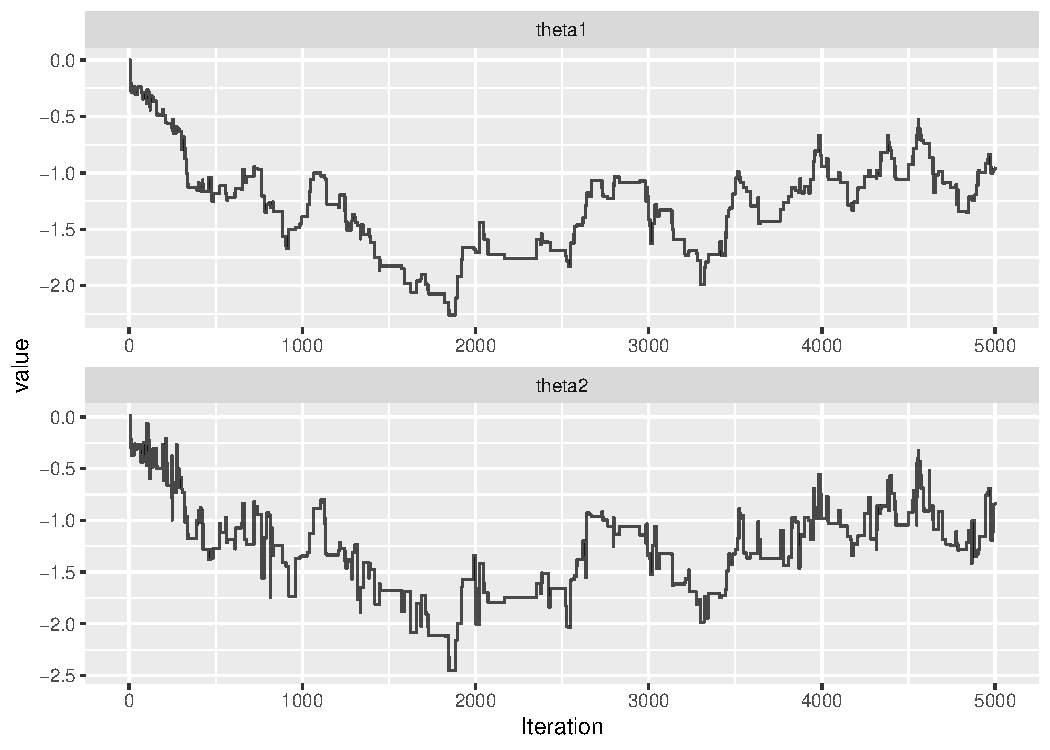
\includegraphics[width=0.8\linewidth]{Bayes_stat_hw3_files/figure-latex/unnamed-chunk-21-1} \end{center}

\paragraph{자기상관계수
그림}\label{uxc790uxae30uxc0c1uxad00uxacc4uxc218-uxadf8uxb9bc-2}

\begin{Shaded}
\begin{Highlighting}[]
\NormalTok{post\_1399 }\SpecialCharTok{\%\textgreater{}\%}\NormalTok{ mcmc }\SpecialCharTok{\%\textgreater{}\%}\NormalTok{ ggs }\SpecialCharTok{\%\textgreater{}\%} \FunctionTok{ggs\_autocorrelation}\NormalTok{()}
\end{Highlighting}
\end{Shaded}

\begin{center}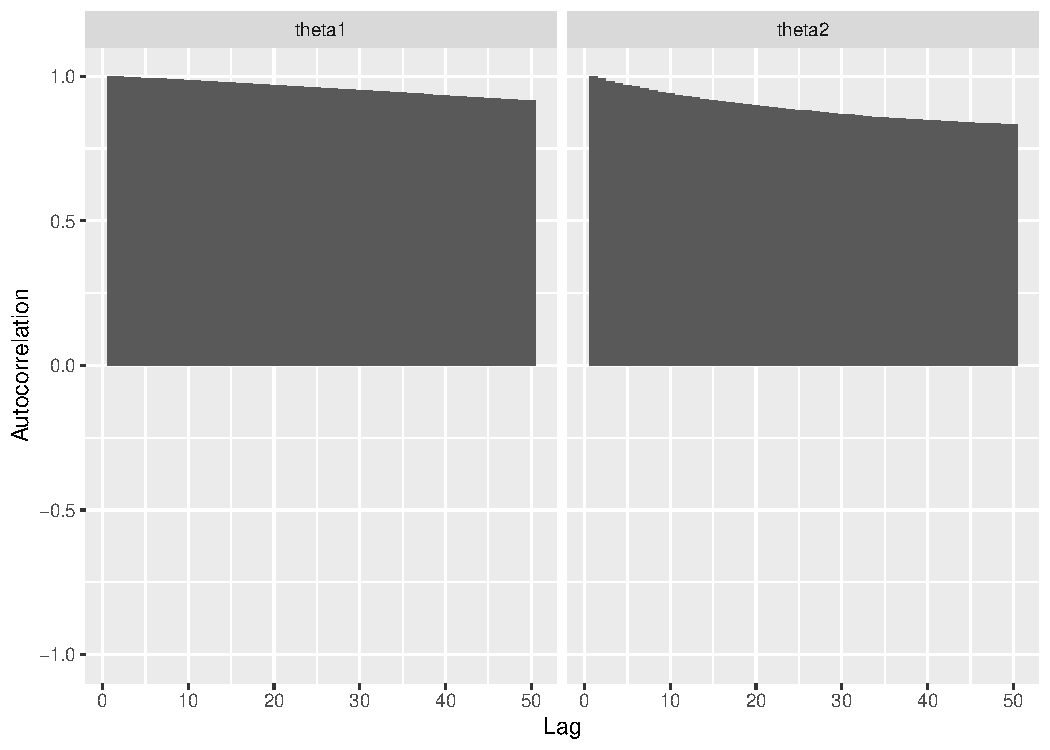
\includegraphics[width=0.8\linewidth]{Bayes_stat_hw3_files/figure-latex/unnamed-chunk-22-1} \end{center}

시계열 자료가 아주 강력하게 패턴을 보인다. 마르코프 체인이 수렴하기 위해
더 많은 반복 수가 필요해 보인다. 20만 회 반복 이후 thining을
시도하였으나 컴퓨터 사양 문제로 실패하였다.

\subsubsection{\texorpdfstring{\(\rho\) =
0.3}{\textbackslash rho = 0.3}}\label{rho-0.3-1}

\begin{Shaded}
\begin{Highlighting}[]
\NormalTok{m }\OtherTok{=} \DecValTok{5000}
\NormalTok{rho }\OtherTok{=} \FloatTok{0.3}
\NormalTok{cov\_mtx }\OtherTok{\textless{}{-}} \FunctionTok{matrix}\NormalTok{(}\FunctionTok{c}\NormalTok{(}\DecValTok{1}\NormalTok{, rho, rho, }\DecValTok{1}\NormalTok{), }\AttributeTok{nrow =} \DecValTok{2}\NormalTok{)}
\NormalTok{d }\OtherTok{=} \FloatTok{0.1}
\NormalTok{po.theta1 }\OtherTok{=} \ConstantTok{NULL}
\NormalTok{po.theta2 }\OtherTok{=} \ConstantTok{NULL}
\NormalTok{theta1 }\OtherTok{=} \DecValTok{0}
\NormalTok{theta2 }\OtherTok{=} \DecValTok{0}
\NormalTok{po.theta1 }\OtherTok{=} \FunctionTok{c}\NormalTok{(po.theta1, theta1)}
\NormalTok{po.theta2 }\OtherTok{=} \FunctionTok{c}\NormalTok{(po.theta2, theta2) }

\FunctionTok{set.seed}\NormalTok{(}\DecValTok{42}\NormalTok{)}
\ControlFlowTok{for}\NormalTok{ (i }\ControlFlowTok{in} \DecValTok{1}\SpecialCharTok{:}\NormalTok{m) \{}\CommentTok{\#m = 5000회 동안 반복.}
\NormalTok{  proposal\_theta1 }\OtherTok{\textless{}{-}} \FunctionTok{rnorm}\NormalTok{(}\DecValTok{1}\NormalTok{, po.theta1[i], d)}
\NormalTok{  proposal\_theta2 }\OtherTok{\textless{}{-}} \FunctionTok{rcauchy}\NormalTok{(}\DecValTok{1}\NormalTok{, }\AttributeTok{location =} \DecValTok{0}\NormalTok{, }\AttributeTok{scale =} \DecValTok{1}\NormalTok{) }\CommentTok{\#제안분포에서 난수 생성}
\NormalTok{  u }\OtherTok{\textless{}{-}} \FunctionTok{runif}\NormalTok{(}\DecValTok{1}\NormalTok{, }\AttributeTok{min =} \DecValTok{0}\NormalTok{, }\AttributeTok{max =} \DecValTok{1}\NormalTok{) }\CommentTok{\#합격{-}불합격 판정용 난수 생성}
\NormalTok{  accp\_prob }\OtherTok{\textless{}{-}} \FunctionTok{min}\NormalTok{(}\DecValTok{1}\NormalTok{, (}\FunctionTok{dmvnorm}\NormalTok{(}\FunctionTok{c}\NormalTok{(proposal\_theta1, proposal\_theta2), }\FunctionTok{c}\NormalTok{(}\DecValTok{0}\NormalTok{, }\DecValTok{0}\NormalTok{), cov\_mtx)}\SpecialCharTok{*}\FunctionTok{dcauchy}\NormalTok{(po.theta2[i], }\DecValTok{0}\NormalTok{, }\DecValTok{1}\NormalTok{))}\SpecialCharTok{/}\NormalTok{(}\FunctionTok{dmvnorm}\NormalTok{(}\FunctionTok{c}\NormalTok{(po.theta1[i], po.theta2[i]), }\FunctionTok{c}\NormalTok{(}\DecValTok{0}\NormalTok{, }\DecValTok{0}\NormalTok{), cov\_mtx)}\SpecialCharTok{*}\FunctionTok{dcauchy}\NormalTok{(proposal\_theta2, }\DecValTok{0}\NormalTok{, }\DecValTok{1}\NormalTok{)))}
  
  \ControlFlowTok{if}\NormalTok{(accp\_prob }\SpecialCharTok{\textgreater{}=}\NormalTok{ u)\{}
\NormalTok{    po.theta1 }\OtherTok{\textless{}{-}} \FunctionTok{c}\NormalTok{(po.theta1, proposal\_theta1)}
\NormalTok{    po.theta2 }\OtherTok{\textless{}{-}} \FunctionTok{c}\NormalTok{(po.theta2, proposal\_theta2)}
\NormalTok{  \} }\ControlFlowTok{else}\NormalTok{\{}
\NormalTok{    po.theta1 }\OtherTok{\textless{}{-}} \FunctionTok{c}\NormalTok{(po.theta1, po.theta1[i])}
\NormalTok{    po.theta2 }\OtherTok{\textless{}{-}} \FunctionTok{c}\NormalTok{(po.theta2, po.theta2[i])}
\NormalTok{  \}}
\NormalTok{\}}

\NormalTok{post\_1303 }\OtherTok{\textless{}{-}} \FunctionTok{data.frame}\NormalTok{(}\AttributeTok{theta1 =}\NormalTok{ po.theta1, }\AttributeTok{theta2 =}\NormalTok{ po.theta2)}
\end{Highlighting}
\end{Shaded}

\paragraph{히스토그램}\label{uxd788uxc2a4uxd1a0uxadf8uxb7a8-3}

\begin{Shaded}
\begin{Highlighting}[]
\NormalTok{post\_1303 }\SpecialCharTok{\%\textgreater{}\%}\NormalTok{ mcmc }\SpecialCharTok{\%\textgreater{}\%}\NormalTok{ ggs }\SpecialCharTok{\%\textgreater{}\%} \FunctionTok{ggs\_histogram}\NormalTok{()}
\end{Highlighting}
\end{Shaded}

\begin{center}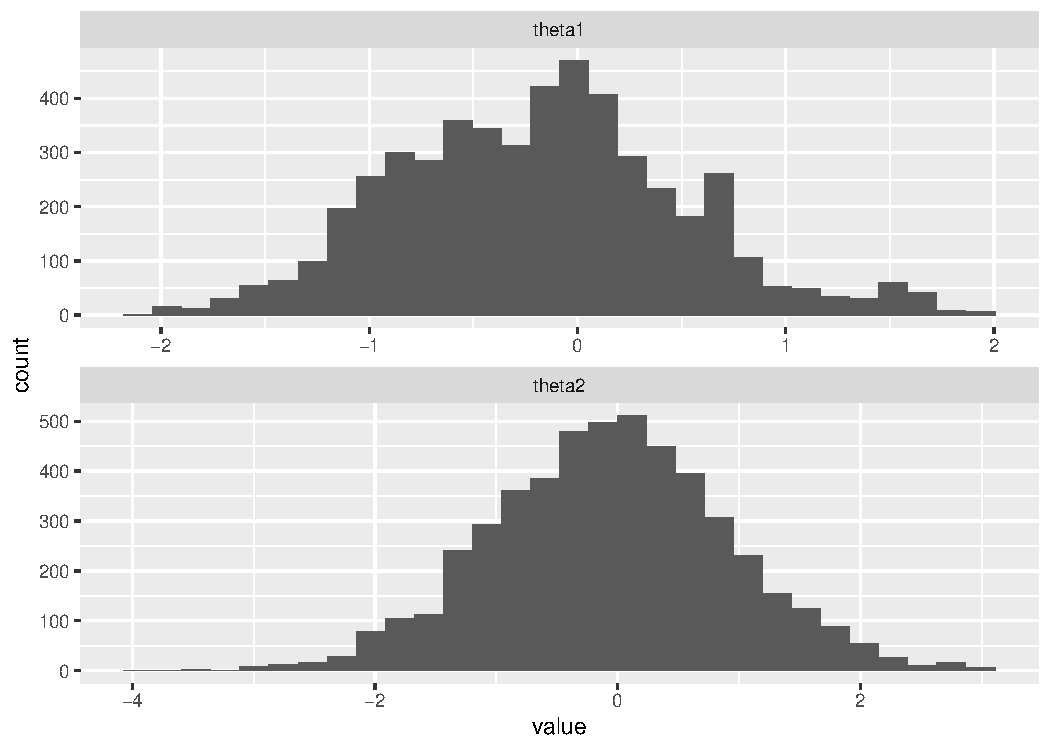
\includegraphics[width=0.8\linewidth]{Bayes_stat_hw3_files/figure-latex/unnamed-chunk-24-1} \end{center}

\begin{Shaded}
\begin{Highlighting}[]
\NormalTok{post\_1303 }\SpecialCharTok{\%\textgreater{}\%}\NormalTok{ mcmc }\SpecialCharTok{\%\textgreater{}\%}\NormalTok{ ggs }\SpecialCharTok{\%\textgreater{}\%} \FunctionTok{ggs\_density}\NormalTok{()}
\end{Highlighting}
\end{Shaded}

\begin{center}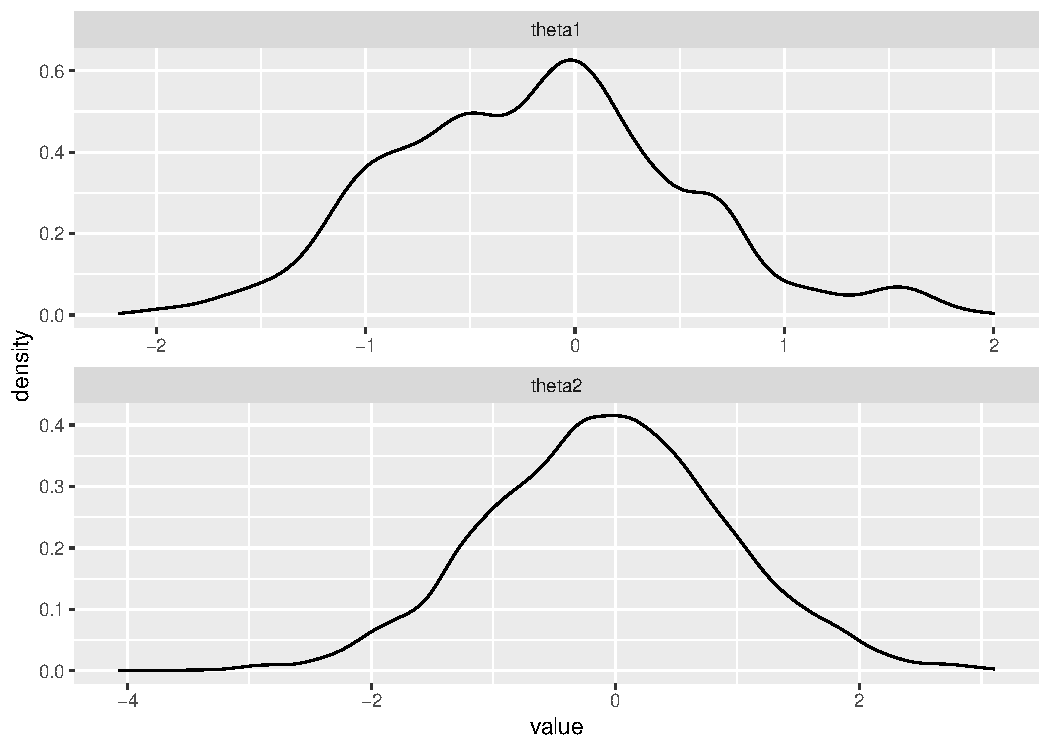
\includegraphics[width=0.8\linewidth]{Bayes_stat_hw3_files/figure-latex/unnamed-chunk-24-2} \end{center}

\paragraph{시계열 그림}\label{uxc2dcuxacc4uxc5f4-uxadf8uxb9bc-3}

\begin{Shaded}
\begin{Highlighting}[]
\NormalTok{post\_1303 }\SpecialCharTok{\%\textgreater{}\%}\NormalTok{ mcmc }\SpecialCharTok{\%\textgreater{}\%}\NormalTok{ ggs }\SpecialCharTok{\%\textgreater{}\%} \FunctionTok{ggs\_traceplot}\NormalTok{()}
\end{Highlighting}
\end{Shaded}

\begin{center}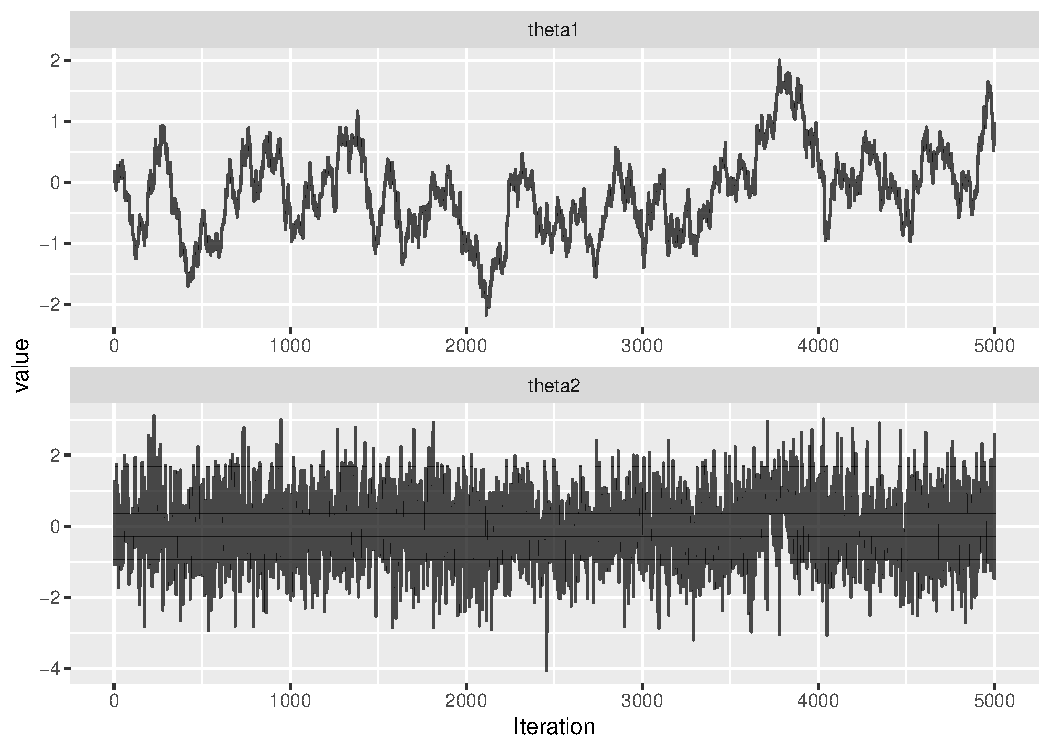
\includegraphics[width=0.8\linewidth]{Bayes_stat_hw3_files/figure-latex/unnamed-chunk-25-1} \end{center}

\paragraph{자기상관계수
그림}\label{uxc790uxae30uxc0c1uxad00uxacc4uxc218-uxadf8uxb9bc-3}

\begin{Shaded}
\begin{Highlighting}[]
\NormalTok{post\_1303 }\SpecialCharTok{\%\textgreater{}\%}\NormalTok{ mcmc }\SpecialCharTok{\%\textgreater{}\%}\NormalTok{ ggs }\SpecialCharTok{\%\textgreater{}\%} \FunctionTok{ggs\_autocorrelation}\NormalTok{()}
\end{Highlighting}
\end{Shaded}

\begin{center}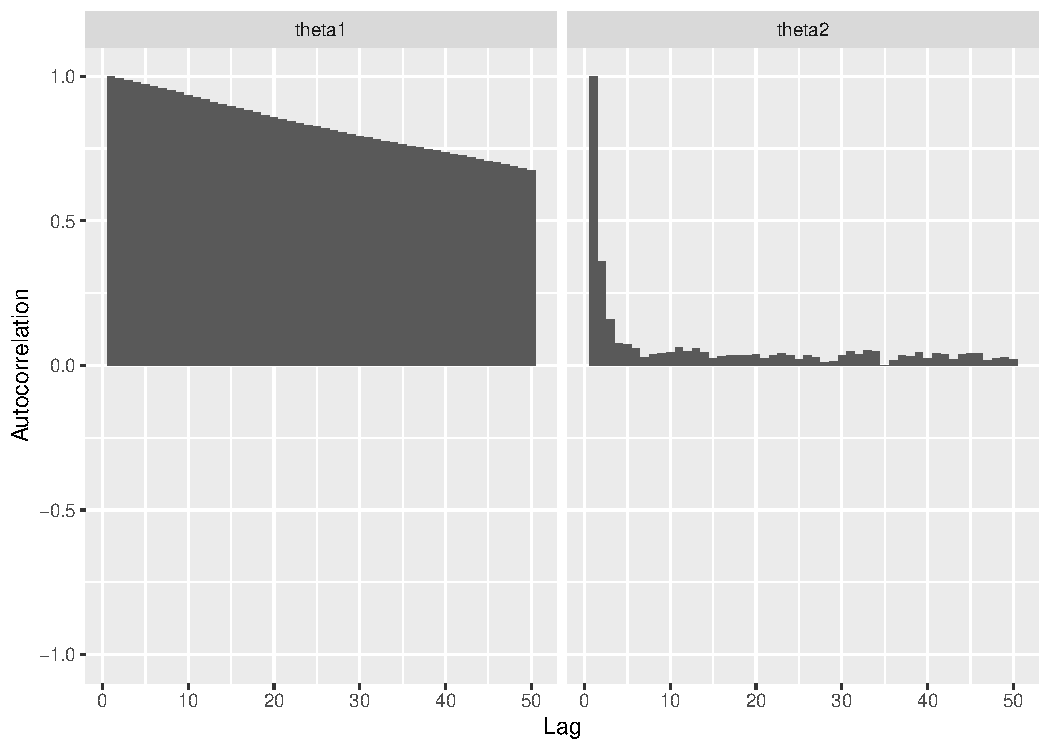
\includegraphics[width=0.8\linewidth]{Bayes_stat_hw3_files/figure-latex/unnamed-chunk-26-1} \end{center}

이 경우, theta2에서는 수렴했다고 볼 수 있으나 theta1에서는 수렴했다고 볼
수 없다.

\subsection{(d)}\label{d-1}

\subsubsection{\texorpdfstring{\(\rho\) =
0.3}{\textbackslash rho = 0.3}}\label{rho-0.3-2}

\begin{Shaded}
\begin{Highlighting}[]
\NormalTok{post\_1303 }\SpecialCharTok{\%\textgreater{}\%}\NormalTok{ mcmc }\SpecialCharTok{\%\textgreater{}\%}\NormalTok{ summary}
\end{Highlighting}
\end{Shaded}

\begin{verbatim}
## 
## Iterations = 1:5001
## Thinning interval = 1 
## Number of chains = 1 
## Sample size per chain = 5001 
## 
## 1. Empirical mean and standard deviation for each variable,
##    plus standard error of the mean:
## 
##            Mean     SD Naive SE Time-series SE
## theta1 -0.18266 0.6894 0.009748         0.1589
## theta2 -0.06557 0.9733 0.013763         0.0256
## 
## 2. Quantiles for each variable:
## 
##          2.5%     25%      50%    75% 97.5%
## theta1 -1.460 -0.6772 -0.17002 0.2410 1.431
## theta2 -1.986 -0.7232 -0.06294 0.5715 1.860
\end{verbatim}

\begin{verbatim}
     2.5%     25%      50%    75% 97.5%    Mean     SD
\end{verbatim}

theta1 -1.460 -0.6772 -0.17002 0.2410 1.431 -0.18266 0.6894 theta2
-1.986 -0.7232 -0.06294 0.5715 1.860 -0.06557 0.9733

\subsubsection{\texorpdfstring{\(\rho\) =
0.3}{\textbackslash rho = 0.3}}\label{rho-0.3-3}

\begin{Shaded}
\begin{Highlighting}[]
\NormalTok{post\_1399 }\SpecialCharTok{\%\textgreater{}\%}\NormalTok{ mcmc }\SpecialCharTok{\%\textgreater{}\%}\NormalTok{ summary}
\end{Highlighting}
\end{Shaded}

\begin{verbatim}
## 
## Iterations = 1:5001
## Thinning interval = 1 
## Number of chains = 1 
## Sample size per chain = 5001 
## 
## 1. Empirical mean and standard deviation for each variable,
##    plus standard error of the mean:
## 
##          Mean     SD Naive SE Time-series SE
## theta1 -1.302 0.4080 0.005770         0.1641
## theta2 -1.292 0.4189 0.005923         0.1158
## 
## 2. Quantiles for each variable:
## 
##          2.5%    25%    50%    75%   97.5%
## theta1 -2.073 -1.634 -1.261 -1.061 -0.3456
## theta2 -2.117 -1.646 -1.278 -1.031 -0.3454
\end{verbatim}

\begin{verbatim}
     2.5%    25%    50%    75%   97.5%  Mean     SD
\end{verbatim}

theta1 -2.073 -1.634 -1.261 -1.061 -0.3456 -1.302 0.4080 theta2 -2.117
-1.646 -1.278 -1.031 -0.3454 -1.292 0.4189

\section{2}\label{section-2}

\subsection{(a)}\label{a-2}

우선 깁스 표본의 개수 m = 5000으로 정한다. 알고리즘의 가동을 확인하기
위해 mu, sig, A에 구체적인 숫자 4, 2, 7을 넣어 확인한다. (b)에서 해당
알고리즘을 표준정규분포에 적용할 것이다.

(단계 1)

\begin{Shaded}
\begin{Highlighting}[]
\NormalTok{m }\OtherTok{=} \DecValTok{5000} \CommentTok{\# 깁스 표본의 수}
\NormalTok{mu }\OtherTok{=} \DecValTok{4} \CommentTok{\# 정규분포의 모평균}
\NormalTok{sig }\OtherTok{=} \DecValTok{2} \CommentTok{\# 정규분포의 모표준편차}
\NormalTok{A }\OtherTok{=} \DecValTok{7} \CommentTok{\# 정규분포의 절단 기준값}
\NormalTok{po.theta }\OtherTok{=} \ConstantTok{NULL} \CommentTok{\# 사후표본을 담을 컨테이너}
\NormalTok{theta\_0 }\OtherTok{=} \FunctionTok{max}\NormalTok{(mu, A }\SpecialCharTok{+} \FloatTok{0.5}\SpecialCharTok{*}\NormalTok{sig) }\CommentTok{\# 초깃값}
\NormalTok{po.theta }\OtherTok{\textless{}{-}} \FunctionTok{c}\NormalTok{(po.theta, theta\_0)}
\end{Highlighting}
\end{Shaded}

(단계 2)

\begin{Shaded}
\begin{Highlighting}[]
\FunctionTok{set.seed}\NormalTok{(}\DecValTok{42}\NormalTok{)}
\ControlFlowTok{for}\NormalTok{ (i }\ControlFlowTok{in} \DecValTok{1}\SpecialCharTok{:}\NormalTok{m) \{}
\NormalTok{  z }\OtherTok{\textless{}{-}} \FunctionTok{runif}\NormalTok{(}\DecValTok{1}\NormalTok{, }\AttributeTok{min =} \DecValTok{0}\NormalTok{, }\AttributeTok{max =} \FunctionTok{exp}\NormalTok{((po.theta[i]}\SpecialCharTok{{-}}\NormalTok{mu)}\SpecialCharTok{\^{}}\DecValTok{2}\SpecialCharTok{/}\NormalTok{(}\SpecialCharTok{{-}}\DecValTok{2}\SpecialCharTok{*}\NormalTok{sig}\SpecialCharTok{\^{}}\DecValTok{2}\NormalTok{)))}
\NormalTok{  t }\OtherTok{\textless{}{-}} \FunctionTok{runif}\NormalTok{(}\DecValTok{1}\NormalTok{, }\FunctionTok{max}\NormalTok{(A, mu }\SpecialCharTok{{-}} \FunctionTok{sqrt}\NormalTok{(}\SpecialCharTok{{-}}\DecValTok{2}\SpecialCharTok{*}\NormalTok{(sig}\SpecialCharTok{\^{}}\DecValTok{2}\NormalTok{)}\SpecialCharTok{*}\FunctionTok{log}\NormalTok{(z))), mu }\SpecialCharTok{+} \FunctionTok{sqrt}\NormalTok{(}\SpecialCharTok{{-}}\DecValTok{2}\SpecialCharTok{*}\NormalTok{(sig}\SpecialCharTok{\^{}}\DecValTok{2}\NormalTok{)}\SpecialCharTok{*}\FunctionTok{log}\NormalTok{(z)))}
\NormalTok{  po.theta }\OtherTok{\textless{}{-}} \FunctionTok{c}\NormalTok{(po.theta, t)}
\NormalTok{\}}
\end{Highlighting}
\end{Shaded}

(단계 3)

\begin{Shaded}
\begin{Highlighting}[]
\FunctionTok{head}\NormalTok{(po.theta)}
\end{Highlighting}
\end{Shaded}

\begin{verbatim}
## [1] 8.000000 8.019607 8.756739 8.098489 7.186747 7.476915
\end{verbatim}

po.theta는 깁스 샘플링으로 생성된 마르코프 체인으로, 절단된 정규분포를
근사한다.

\subsection{(b)}\label{b-2}

우선 문제를 풀기 위해 (a)의 알고리즘을 함수로 묶자. \(\mu\) = 0,
\(\sigma\) = 1을 고정하고, 표본 추출 수 k와 절단 위치 a를 인자로 받아
표본 추출 결과 데이터프레임을 return하는 함수를 만들면 된다.

\begin{Shaded}
\begin{Highlighting}[]
\NormalTok{gibbs\_truncated\_normal }\OtherTok{\textless{}{-}} \ControlFlowTok{function}\NormalTok{(k, a)\{}
\NormalTok{  m }\OtherTok{=}\NormalTok{ k }\CommentTok{\# 깁스 표본의 수}
\NormalTok{  mu }\OtherTok{=} \DecValTok{0} 
\NormalTok{  sig }\OtherTok{=} \DecValTok{1} 
\NormalTok{  A }\OtherTok{=}\NormalTok{ a }
\NormalTok{  po.theta }\OtherTok{=} \ConstantTok{NULL} \CommentTok{\# 사후표본을 담을 컨테이너}
\NormalTok{  theta\_0 }\OtherTok{=} \FunctionTok{max}\NormalTok{(mu, A }\SpecialCharTok{+} \FloatTok{0.5}\SpecialCharTok{*}\NormalTok{sig) }\CommentTok{\# 초깃값}
\NormalTok{  po.theta }\OtherTok{\textless{}{-}} \FunctionTok{c}\NormalTok{(po.theta, theta\_0)}

  \FunctionTok{set.seed}\NormalTok{(}\DecValTok{42}\NormalTok{)}
  \ControlFlowTok{for}\NormalTok{ (i }\ControlFlowTok{in} \DecValTok{1}\SpecialCharTok{:}\NormalTok{m) \{}
\NormalTok{    z }\OtherTok{\textless{}{-}} \FunctionTok{runif}\NormalTok{(}\DecValTok{1}\NormalTok{, }\AttributeTok{min =} \DecValTok{0}\NormalTok{, }\AttributeTok{max =} \FunctionTok{exp}\NormalTok{((po.theta[i]}\SpecialCharTok{{-}}\NormalTok{mu)}\SpecialCharTok{\^{}}\DecValTok{2}\SpecialCharTok{/}\NormalTok{(}\SpecialCharTok{{-}}\DecValTok{2}\SpecialCharTok{*}\NormalTok{sig}\SpecialCharTok{\^{}}\DecValTok{2}\NormalTok{)))}
\NormalTok{    t }\OtherTok{\textless{}{-}} \FunctionTok{runif}\NormalTok{(}\DecValTok{1}\NormalTok{, }\FunctionTok{max}\NormalTok{(A, mu }\SpecialCharTok{{-}} \FunctionTok{sqrt}\NormalTok{(}\SpecialCharTok{{-}}\DecValTok{2}\SpecialCharTok{*}\NormalTok{(sig}\SpecialCharTok{\^{}}\DecValTok{2}\NormalTok{)}\SpecialCharTok{*}\FunctionTok{log}\NormalTok{(z))), mu }\SpecialCharTok{+} \FunctionTok{sqrt}\NormalTok{(}\SpecialCharTok{{-}}\DecValTok{2}\SpecialCharTok{*}\NormalTok{(sig}\SpecialCharTok{\^{}}\DecValTok{2}\NormalTok{)}\SpecialCharTok{*}\FunctionTok{log}\NormalTok{(z)))}
\NormalTok{    po.theta }\OtherTok{\textless{}{-}} \FunctionTok{c}\NormalTok{(po.theta, t)}
\NormalTok{  \}}
\NormalTok{  df\_gi }\OtherTok{\textless{}{-}} \FunctionTok{data.frame}\NormalTok{(}\AttributeTok{theta =}\NormalTok{ po.theta)}
  \FunctionTok{return}\NormalTok{(df\_gi)}
\NormalTok{\}}
\end{Highlighting}
\end{Shaded}

\subsubsection{A = 1}\label{a-1-1}

\begin{Shaded}
\begin{Highlighting}[]
\NormalTok{post\_201\_5000 }\OtherTok{\textless{}{-}} \FunctionTok{gibbs\_truncated\_normal}\NormalTok{(}\DecValTok{5000}\NormalTok{, }\DecValTok{1}\NormalTok{)}
\end{Highlighting}
\end{Shaded}

(m = 5000)

\begin{Shaded}
\begin{Highlighting}[]
\NormalTok{post\_201\_5000 }\SpecialCharTok{\%\textgreater{}\%}\NormalTok{ mcmc }\SpecialCharTok{\%\textgreater{}\%}\NormalTok{ ggs }\SpecialCharTok{\%\textgreater{}\%} \FunctionTok{ggs\_traceplot}\NormalTok{()}
\end{Highlighting}
\end{Shaded}

\begin{center}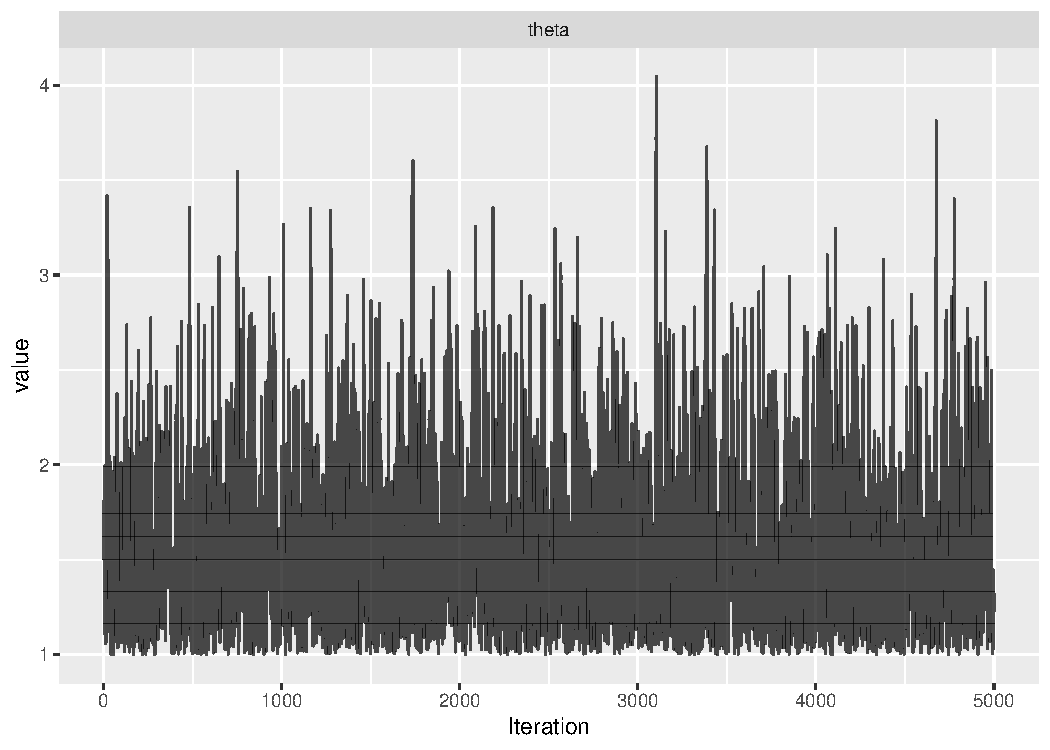
\includegraphics[width=0.8\linewidth]{Bayes_stat_hw3_files/figure-latex/unnamed-chunk-34-1} \end{center}

\begin{Shaded}
\begin{Highlighting}[]
\NormalTok{post\_201\_5000 }\SpecialCharTok{\%\textgreater{}\%}\NormalTok{ mcmc }\SpecialCharTok{\%\textgreater{}\%}\NormalTok{ ggs }\SpecialCharTok{\%\textgreater{}\%} \FunctionTok{ggs\_autocorrelation}\NormalTok{()}
\end{Highlighting}
\end{Shaded}

\begin{center}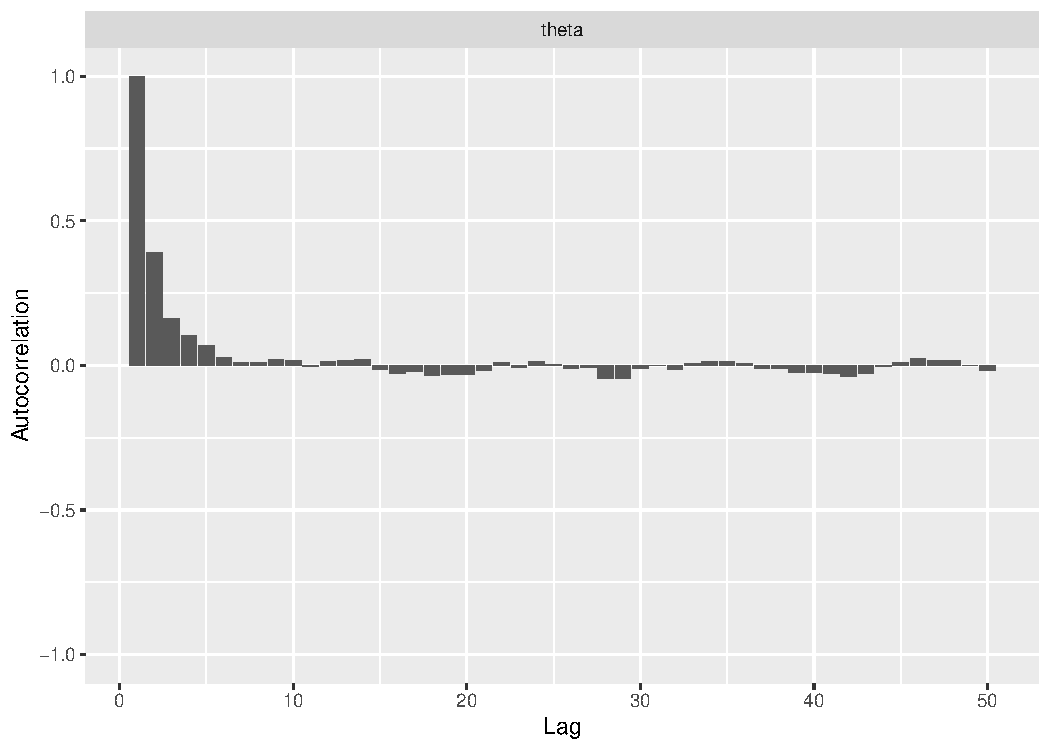
\includegraphics[width=0.8\linewidth]{Bayes_stat_hw3_files/figure-latex/unnamed-chunk-34-2} \end{center}

m = 5000에서도 충분히 수렴했다고 판단할 수 있다.

\subsubsection{A = 5}\label{a-5}

\begin{Shaded}
\begin{Highlighting}[]
\NormalTok{post\_205\_5000 }\OtherTok{\textless{}{-}} \FunctionTok{gibbs\_truncated\_normal}\NormalTok{(}\DecValTok{5000}\NormalTok{, }\DecValTok{5}\NormalTok{)}
\end{Highlighting}
\end{Shaded}

(m = 5000)

\begin{Shaded}
\begin{Highlighting}[]
\NormalTok{post\_205\_5000 }\SpecialCharTok{\%\textgreater{}\%}\NormalTok{ mcmc }\SpecialCharTok{\%\textgreater{}\%}\NormalTok{ ggs }\SpecialCharTok{\%\textgreater{}\%} \FunctionTok{ggs\_density}\NormalTok{()}
\end{Highlighting}
\end{Shaded}

\begin{center}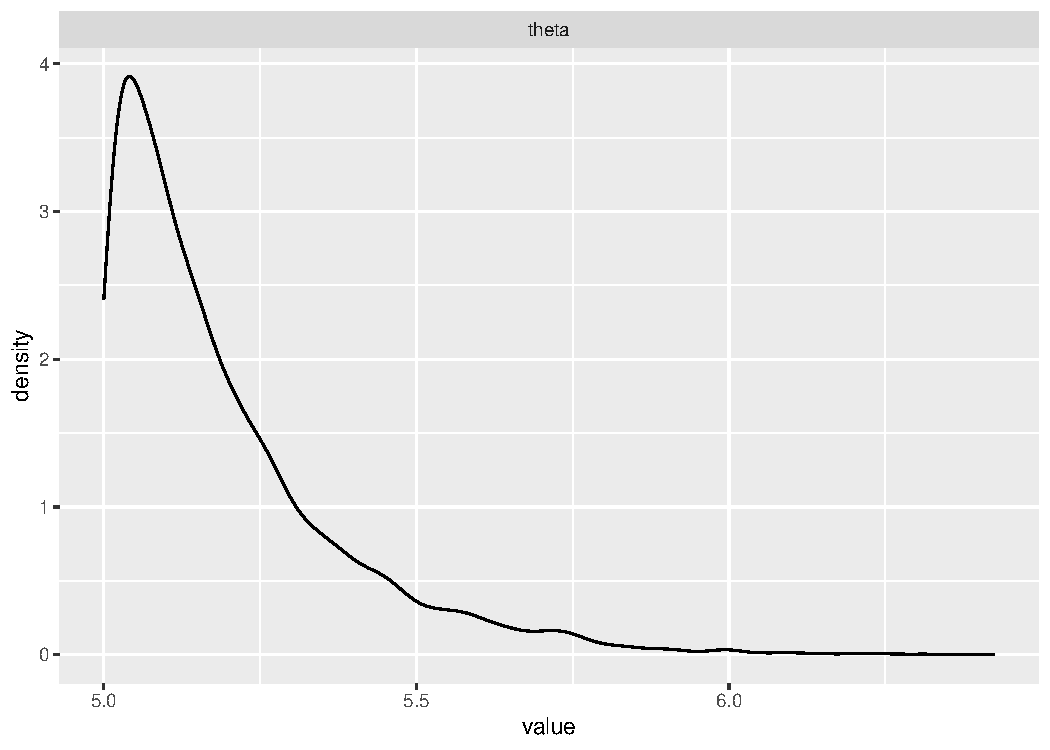
\includegraphics[width=0.8\linewidth]{Bayes_stat_hw3_files/figure-latex/unnamed-chunk-36-1} \end{center}

\begin{Shaded}
\begin{Highlighting}[]
\NormalTok{post\_205\_5000 }\SpecialCharTok{\%\textgreater{}\%}\NormalTok{ mcmc }\SpecialCharTok{\%\textgreater{}\%}\NormalTok{ ggs }\SpecialCharTok{\%\textgreater{}\%} \FunctionTok{ggs\_traceplot}\NormalTok{()}
\end{Highlighting}
\end{Shaded}

\begin{center}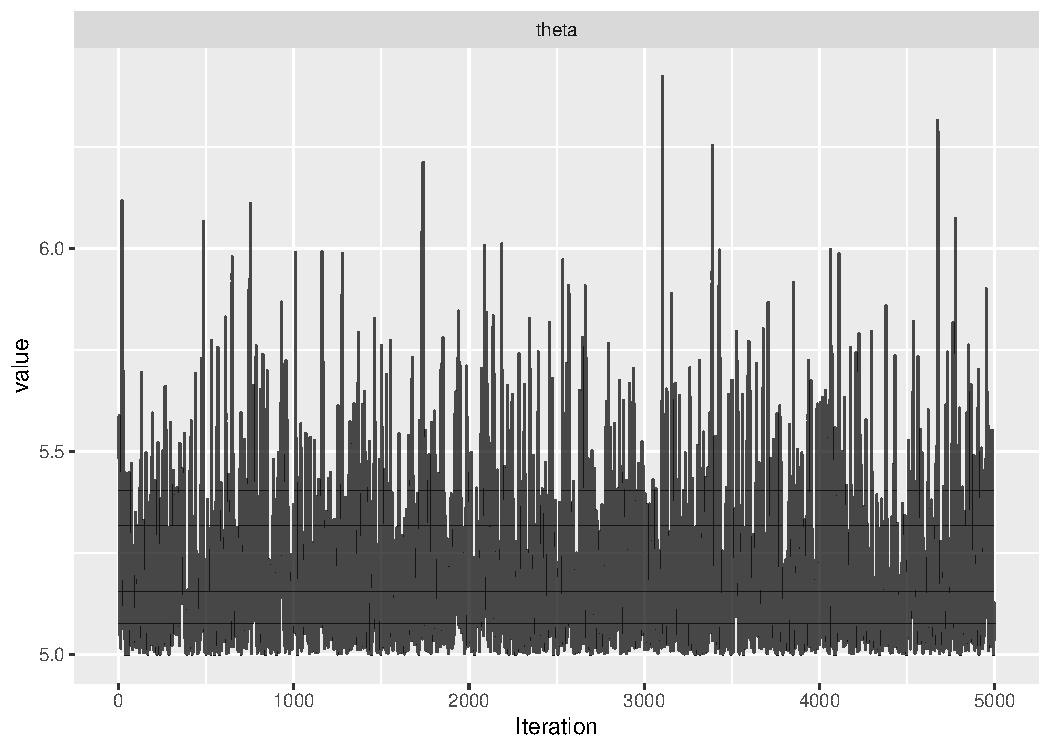
\includegraphics[width=0.8\linewidth]{Bayes_stat_hw3_files/figure-latex/unnamed-chunk-36-2} \end{center}

\begin{Shaded}
\begin{Highlighting}[]
\NormalTok{post\_205\_5000 }\SpecialCharTok{\%\textgreater{}\%}\NormalTok{ mcmc }\SpecialCharTok{\%\textgreater{}\%}\NormalTok{ ggs }\SpecialCharTok{\%\textgreater{}\%} \FunctionTok{ggs\_autocorrelation}\NormalTok{()}
\end{Highlighting}
\end{Shaded}

\begin{center}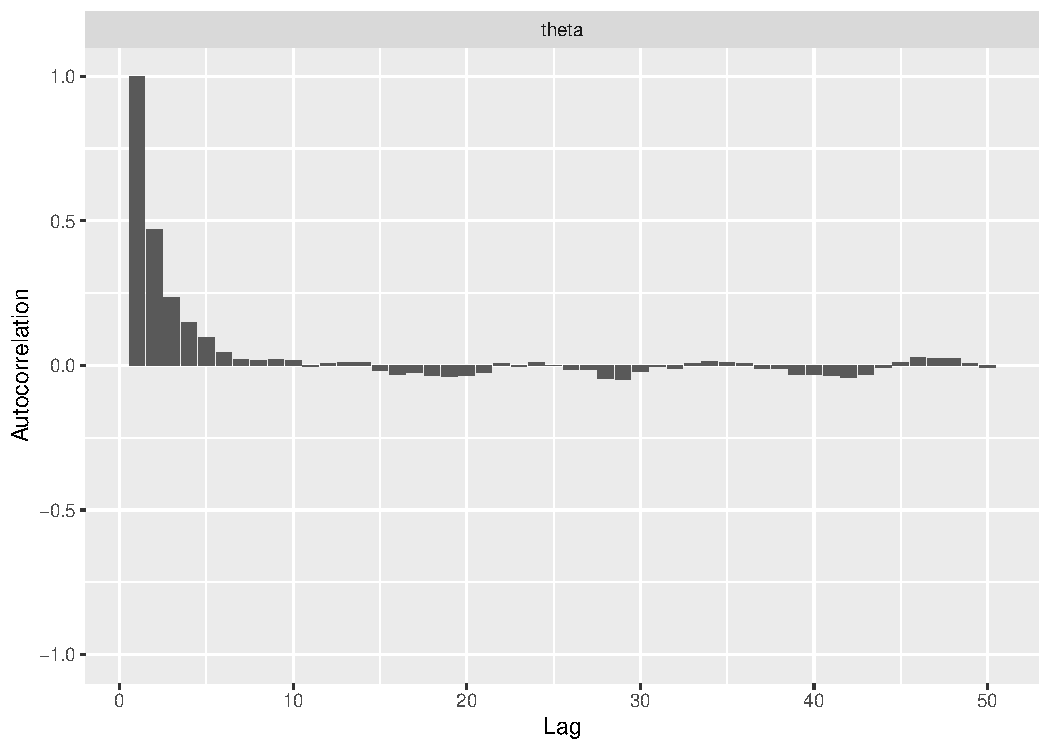
\includegraphics[width=0.8\linewidth]{Bayes_stat_hw3_files/figure-latex/unnamed-chunk-36-3} \end{center}

m = 5000에서 충분히 수렴했다고 판단할 수 있다.

\subsubsection{A = 10}\label{a-10}

\begin{Shaded}
\begin{Highlighting}[]
\NormalTok{post\_210\_5000 }\OtherTok{\textless{}{-}} \FunctionTok{gibbs\_truncated\_normal}\NormalTok{(}\DecValTok{5000}\NormalTok{, }\DecValTok{10}\NormalTok{)}
\NormalTok{post\_210\_1000 }\OtherTok{\textless{}{-}} \FunctionTok{gibbs\_truncated\_normal}\NormalTok{(}\DecValTok{1000}\NormalTok{, }\DecValTok{10}\NormalTok{)}
\end{Highlighting}
\end{Shaded}

(m = 1000)

\begin{Shaded}
\begin{Highlighting}[]
\NormalTok{post\_210\_1000 }\SpecialCharTok{\%\textgreater{}\%}\NormalTok{ mcmc }\SpecialCharTok{\%\textgreater{}\%}\NormalTok{ ggs }\SpecialCharTok{\%\textgreater{}\%} \FunctionTok{ggs\_density}\NormalTok{()}
\end{Highlighting}
\end{Shaded}

\begin{center}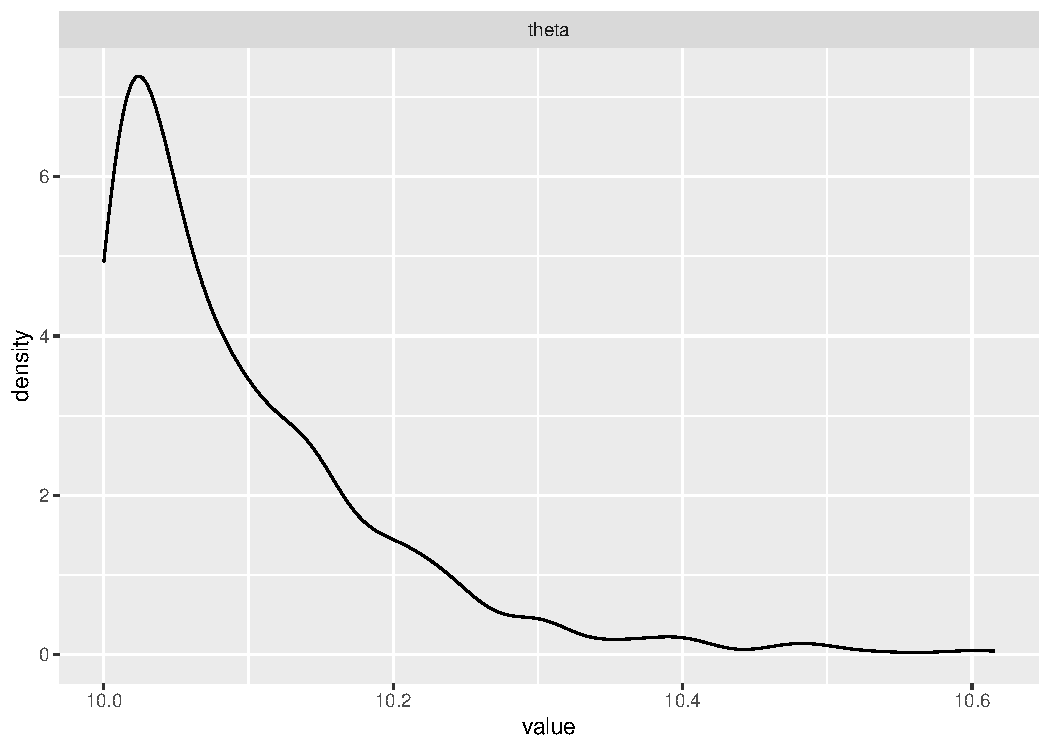
\includegraphics[width=0.8\linewidth]{Bayes_stat_hw3_files/figure-latex/unnamed-chunk-38-1} \end{center}

\begin{Shaded}
\begin{Highlighting}[]
\NormalTok{post\_210\_1000 }\SpecialCharTok{\%\textgreater{}\%}\NormalTok{ mcmc }\SpecialCharTok{\%\textgreater{}\%}\NormalTok{ ggs }\SpecialCharTok{\%\textgreater{}\%} \FunctionTok{ggs\_traceplot}\NormalTok{()}
\end{Highlighting}
\end{Shaded}

\begin{center}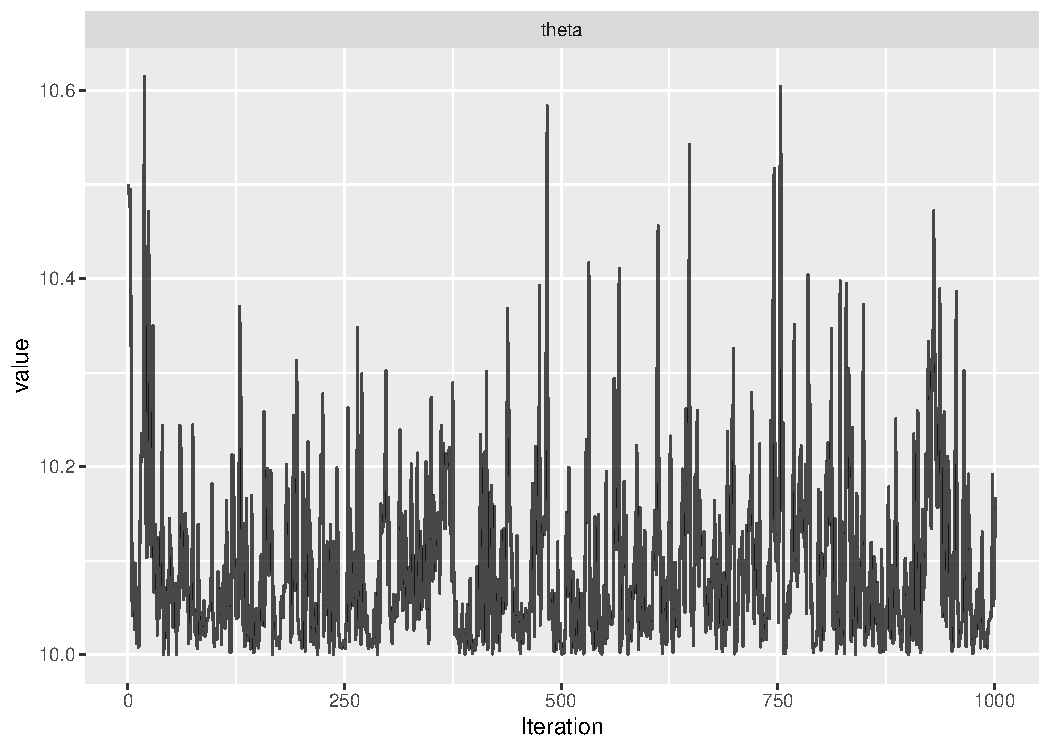
\includegraphics[width=0.8\linewidth]{Bayes_stat_hw3_files/figure-latex/unnamed-chunk-38-2} \end{center}

\begin{Shaded}
\begin{Highlighting}[]
\NormalTok{post\_210\_1000 }\SpecialCharTok{\%\textgreater{}\%}\NormalTok{ mcmc }\SpecialCharTok{\%\textgreater{}\%}\NormalTok{ ggs }\SpecialCharTok{\%\textgreater{}\%} \FunctionTok{ggs\_autocorrelation}\NormalTok{()}
\end{Highlighting}
\end{Shaded}

\begin{center}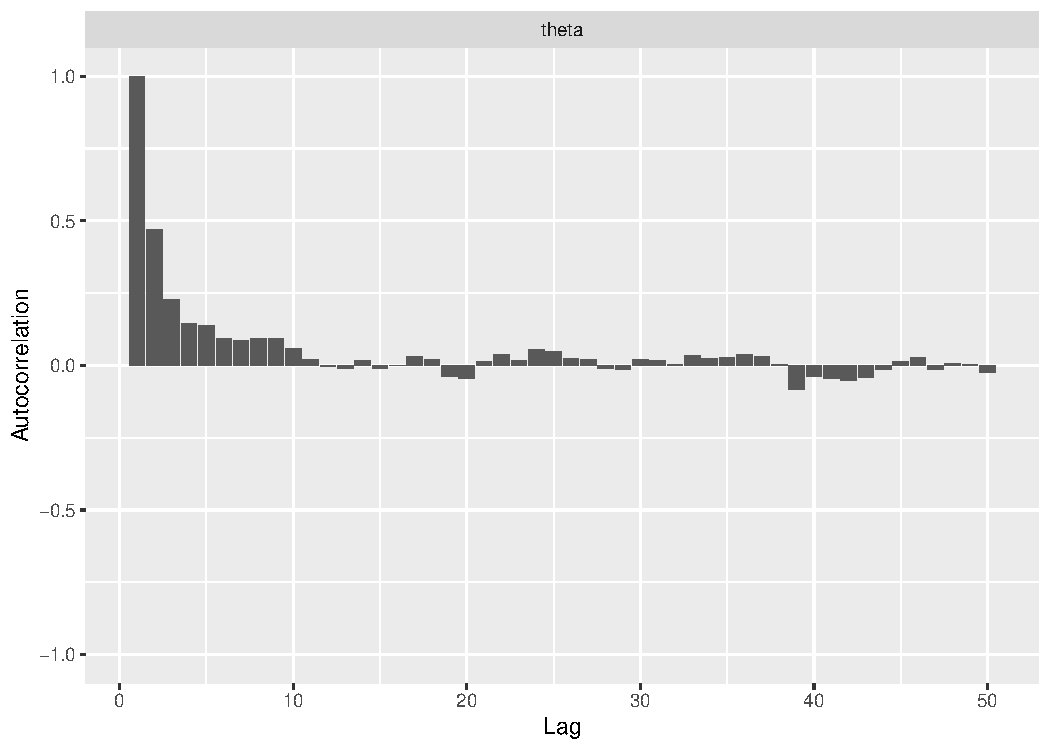
\includegraphics[width=0.8\linewidth]{Bayes_stat_hw3_files/figure-latex/unnamed-chunk-38-3} \end{center}

(m = 5000)

\begin{Shaded}
\begin{Highlighting}[]
\NormalTok{post\_210\_5000 }\SpecialCharTok{\%\textgreater{}\%}\NormalTok{ mcmc }\SpecialCharTok{\%\textgreater{}\%}\NormalTok{ ggs }\SpecialCharTok{\%\textgreater{}\%} \FunctionTok{ggs\_density}\NormalTok{()}
\end{Highlighting}
\end{Shaded}

\begin{center}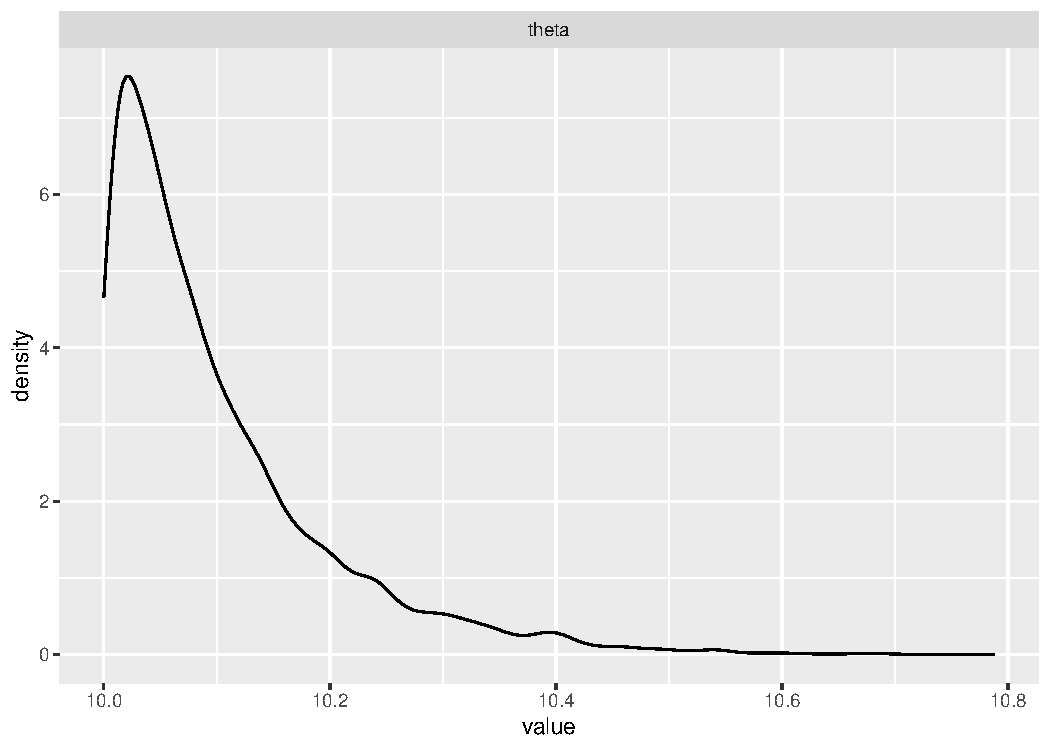
\includegraphics[width=0.8\linewidth]{Bayes_stat_hw3_files/figure-latex/unnamed-chunk-39-1} \end{center}

\begin{Shaded}
\begin{Highlighting}[]
\NormalTok{post\_210\_5000 }\SpecialCharTok{\%\textgreater{}\%}\NormalTok{ mcmc }\SpecialCharTok{\%\textgreater{}\%}\NormalTok{ ggs }\SpecialCharTok{\%\textgreater{}\%} \FunctionTok{ggs\_traceplot}\NormalTok{()}
\end{Highlighting}
\end{Shaded}

\begin{center}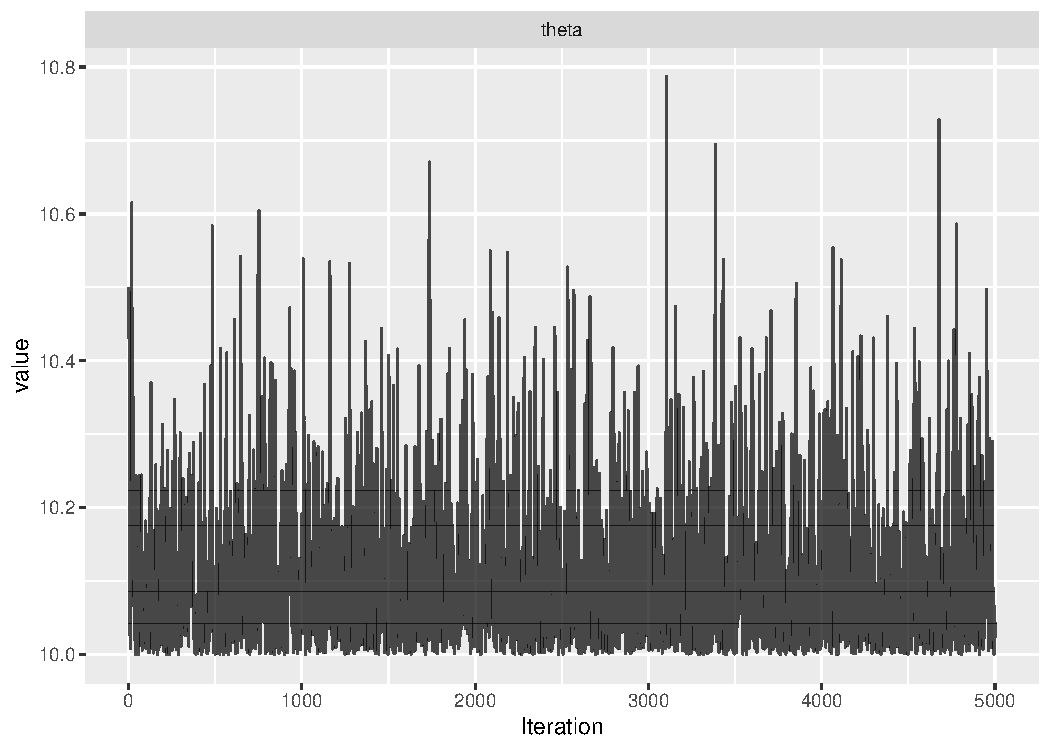
\includegraphics[width=0.8\linewidth]{Bayes_stat_hw3_files/figure-latex/unnamed-chunk-39-2} \end{center}

\begin{Shaded}
\begin{Highlighting}[]
\NormalTok{post\_210\_5000 }\SpecialCharTok{\%\textgreater{}\%}\NormalTok{ mcmc }\SpecialCharTok{\%\textgreater{}\%}\NormalTok{ ggs }\SpecialCharTok{\%\textgreater{}\%} \FunctionTok{ggs\_autocorrelation}\NormalTok{()}
\end{Highlighting}
\end{Shaded}

\begin{center}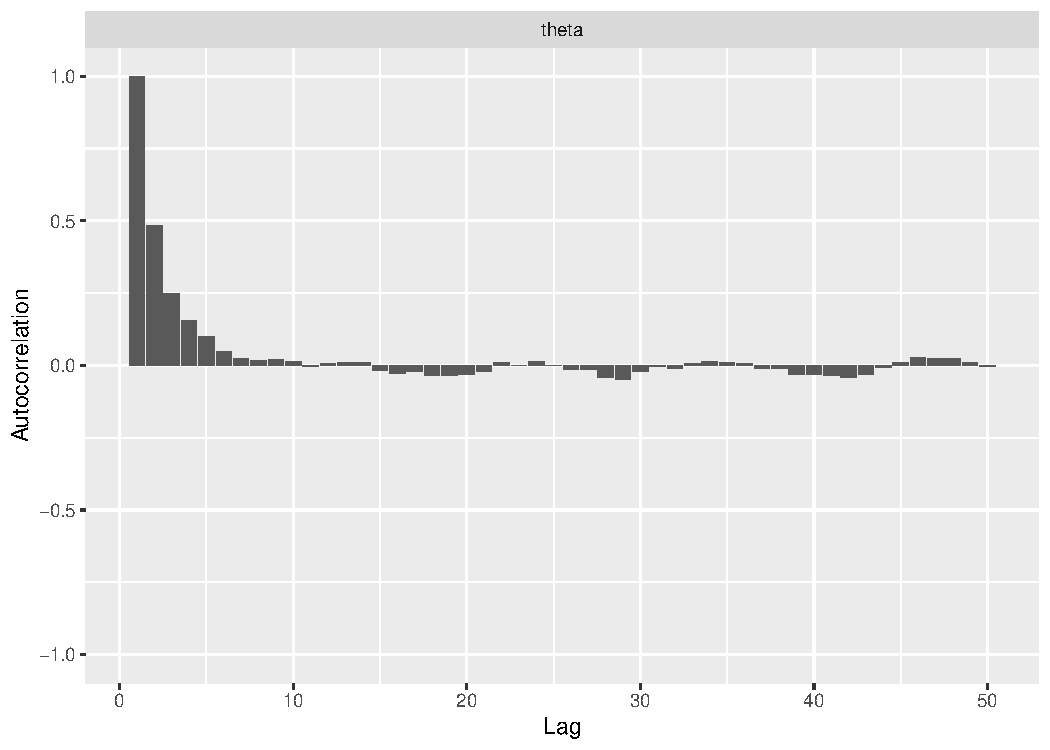
\includegraphics[width=0.8\linewidth]{Bayes_stat_hw3_files/figure-latex/unnamed-chunk-39-3} \end{center}

m = 5000에서 수렴했다고 충분히 판단할 수 있다. m = 1000인 경우를 보면
수렴하지 않은 경우 '경향성'이 있음을 확연히 알 수 있다.

\subsection{(c)}\label{c-2}

\subsubsection{A = 1}\label{a-1-2}

\begin{Shaded}
\begin{Highlighting}[]
\NormalTok{post\_201\_5000 }\SpecialCharTok{\%\textgreater{}\%}\NormalTok{ mcmc }\SpecialCharTok{\%\textgreater{}\%}\NormalTok{ summary}
\end{Highlighting}
\end{Shaded}

\begin{verbatim}
## 
## Iterations = 1:5001
## Thinning interval = 1 
## Number of chains = 1 
## Sample size per chain = 5001 
## 
## 1. Empirical mean and standard deviation for each variable,
##    plus standard error of the mean:
## 
##           Mean             SD       Naive SE Time-series SE 
##        1.52968        0.45398        0.00642        0.01026 
## 
## 2. Quantiles for each variable:
## 
##  2.5%   25%   50%   75% 97.5% 
## 1.016 1.178 1.410 1.757 2.704
\end{verbatim}

\begin{verbatim}
   2.5%   25%   50%   75% 97.5%    Mean      SD
\end{verbatim}

theta 1.016 1.178 1.410 1.757 2.704 1.52968 0.45398

\subsubsection{A = 5}\label{a-5-1}

\begin{Shaded}
\begin{Highlighting}[]
\NormalTok{post\_205\_5000 }\SpecialCharTok{\%\textgreater{}\%}\NormalTok{ mcmc }\SpecialCharTok{\%\textgreater{}\%}\NormalTok{ summary}
\end{Highlighting}
\end{Shaded}

\begin{verbatim}
## 
## Iterations = 1:5001
## Thinning interval = 1 
## Number of chains = 1 
## Sample size per chain = 5001 
## 
## 1. Empirical mean and standard deviation for each variable,
##    plus standard error of the mean:
## 
##           Mean             SD       Naive SE Time-series SE 
##       5.188972       0.184461       0.002608       0.004613 
## 
## 2. Quantiles for each variable:
## 
##  2.5%   25%   50%   75% 97.5% 
## 5.004 5.056 5.133 5.261 5.697
\end{verbatim}

\begin{verbatim}
   2.5%   25%   50%   75% 97.5%     Mean       SD
\end{verbatim}

theta 5.004 5.056 5.133 5.261 5.697 5.188972 0.184461

\subsubsection{A = 10}\label{a-10-1}

\begin{Shaded}
\begin{Highlighting}[]
\NormalTok{post\_210\_5000 }\SpecialCharTok{\%\textgreater{}\%}\NormalTok{ mcmc }\SpecialCharTok{\%\textgreater{}\%}\NormalTok{ summary}
\end{Highlighting}
\end{Shaded}

\begin{verbatim}
## 
## Iterations = 1:5001
## Thinning interval = 1 
## Number of chains = 1 
## Sample size per chain = 5001 
## 
## 1. Empirical mean and standard deviation for each variable,
##    plus standard error of the mean:
## 
##           Mean             SD       Naive SE Time-series SE 
##      10.099615       0.099508       0.001407       0.002524 
## 
## 2. Quantiles for each variable:
## 
##  2.5%   25%   50%   75% 97.5% 
## 10.00 10.03 10.07 10.14 10.38
\end{verbatim}

\begin{verbatim}
   2.5%   25%   50%   75% 97.5%     Mean        SD
\end{verbatim}

theta 10.00 10.03 10.07 10.14 10.38 10.099615 0.099508

\section{3}\label{section-3}

\subsection{(a)}\label{a-3}

해당 문제는 종이에 풀이하였다.

\subsection{(b)}\label{b-3}

해당 문제는 종이에 풀이하였다.

\subsection{(c)}\label{c-3}

\subsubsection{초깃값}\label{uxcd08uxae43uxac12}

\begin{Shaded}
\begin{Highlighting}[]
\NormalTok{df }\OtherTok{\textless{}{-}} \FunctionTok{c}\NormalTok{(}\FloatTok{68.3}\NormalTok{, }\FloatTok{85.7}\NormalTok{, }\FloatTok{73.8}\NormalTok{, }\FloatTok{83.2}\NormalTok{, }\FloatTok{58.9}\NormalTok{, }\FloatTok{72.7}\NormalTok{, }\FloatTok{70.5}\NormalTok{, }\FloatTok{58.7}\NormalTok{, }\FloatTok{74.1}\NormalTok{, }\FloatTok{75.0}\NormalTok{) }\CommentTok{\#가능도}
\NormalTok{m }\OtherTok{\textless{}{-}} \DecValTok{5000}
\NormalTok{nu }\OtherTok{\textless{}{-}} \DecValTok{20} \CommentTok{\#prior의 정보 1}
\NormalTok{theta0 }\OtherTok{\textless{}{-}} \DecValTok{0} \CommentTok{\#prior의 정보 2}
\NormalTok{nu0 }\OtherTok{\textless{}{-}} \DecValTok{1} \CommentTok{\#prior의 정보 3}
\NormalTok{s02 }\OtherTok{\textless{}{-}} \DecValTok{1} \CommentTok{\#prior의 정보 4}
\NormalTok{theta\_0 }\OtherTok{\textless{}{-}} \DecValTok{0}
\NormalTok{delta\_0 }\OtherTok{\textless{}{-}} \DecValTok{1}
\NormalTok{ksi\_0 }\OtherTok{\textless{}{-}} \DecValTok{0}
\NormalTok{po.theta }\OtherTok{=} \ConstantTok{NULL}
\NormalTok{po.delta }\OtherTok{=} \ConstantTok{NULL}
\NormalTok{po.ksi }\OtherTok{=} \ConstantTok{NULL}
\NormalTok{po.theta }\OtherTok{\textless{}{-}} \FunctionTok{c}\NormalTok{(po.theta, theta\_0)}
\NormalTok{po.delta }\OtherTok{\textless{}{-}} \FunctionTok{c}\NormalTok{(po.delta, delta\_0)}
\NormalTok{po.ksi }\OtherTok{\textless{}{-}} \FunctionTok{c}\NormalTok{(po.ksi, ksi\_0)}
\end{Highlighting}
\end{Shaded}

\subsubsection{깁스 샘플링
반복}\label{uxae41uxc2a4-uxc0d8uxd50cuxb9c1-uxbc18uxbcf5}

\begin{Shaded}
\begin{Highlighting}[]
\FunctionTok{set.seed}\NormalTok{(}\DecValTok{42}\NormalTok{)}
\ControlFlowTok{for}\NormalTok{ (i }\ControlFlowTok{in} \DecValTok{1}\SpecialCharTok{:}\NormalTok{m) \{}
\NormalTok{  ksi\_prime }\OtherTok{\textless{}{-}} \FunctionTok{rgamma}\NormalTok{(}\DecValTok{1}\NormalTok{, (}\DecValTok{1}\SpecialCharTok{+}\NormalTok{nu)}\SpecialCharTok{/}\DecValTok{2}\NormalTok{, }\AttributeTok{rate =} \DecValTok{1} \SpecialCharTok{+}\NormalTok{ ((po.theta[i]}\SpecialCharTok{{-}}\NormalTok{theta0)}\SpecialCharTok{\^{}}\DecValTok{2}\NormalTok{) }\SpecialCharTok{/}\NormalTok{ (nu}\SpecialCharTok{*}\NormalTok{po.delta[i]))}
\NormalTok{  theta\_prime }\OtherTok{\textless{}{-}} \FunctionTok{rnorm}\NormalTok{(}\DecValTok{1}\NormalTok{, (nu}\SpecialCharTok{*}\FunctionTok{mean}\NormalTok{(df) }\SpecialCharTok{+} \DecValTok{2}\SpecialCharTok{*}\NormalTok{theta0}\SpecialCharTok{*}\NormalTok{ksi\_prime) }\SpecialCharTok{/}\NormalTok{ (nu}\SpecialCharTok{+}\DecValTok{2}\SpecialCharTok{*}\NormalTok{ksi\_prime), }\FunctionTok{sqrt}\NormalTok{((nu}\SpecialCharTok{*}\NormalTok{po.delta[i]) }\SpecialCharTok{/}\NormalTok{ (nu}\SpecialCharTok{+}\DecValTok{2}\SpecialCharTok{*}\NormalTok{ksi\_prime)))}
\NormalTok{  delta\_rate }\OtherTok{=}\NormalTok{ (((nu }\SpecialCharTok{+} \DecValTok{2}\SpecialCharTok{*}\NormalTok{ksi\_prime)}\SpecialCharTok{*}\NormalTok{((theta\_prime }\SpecialCharTok{{-}}\NormalTok{ (nu}\SpecialCharTok{*}\FunctionTok{mean}\NormalTok{(df) }\SpecialCharTok{+} \DecValTok{2}\SpecialCharTok{*}\NormalTok{ksi\_prime}\SpecialCharTok{*}\NormalTok{theta0) }\SpecialCharTok{/}\NormalTok{ (nu }\SpecialCharTok{+} \DecValTok{2}\SpecialCharTok{*}\NormalTok{ksi\_prime))}\SpecialCharTok{\^{}}\DecValTok{2}\NormalTok{))}\SpecialCharTok{/}\NormalTok{(}\DecValTok{2}\SpecialCharTok{*}\NormalTok{nu))}\SpecialCharTok{+}\NormalTok{(}\DecValTok{1}\SpecialCharTok{/}\DecValTok{2}\NormalTok{)}\SpecialCharTok{*}\NormalTok{(nu0}\SpecialCharTok{*}\NormalTok{s02}\SpecialCharTok{+}\NormalTok{(}\FunctionTok{length}\NormalTok{(df)}\SpecialCharTok{{-}}\DecValTok{1}\NormalTok{)}\SpecialCharTok{*}\FunctionTok{var}\NormalTok{(df)}\SpecialCharTok{+}\NormalTok{(}\DecValTok{2}\SpecialCharTok{*}\NormalTok{ksi\_prime}\SpecialCharTok{*}\NormalTok{(}\FunctionTok{mean}\NormalTok{(df)}\SpecialCharTok{{-}}\NormalTok{theta0)}\SpecialCharTok{\^{}}\DecValTok{2}\NormalTok{)}\SpecialCharTok{/}\NormalTok{(nu}\SpecialCharTok{+}\DecValTok{2}\SpecialCharTok{*}\NormalTok{ksi\_prime))}
\NormalTok{  delta\_prime }\OtherTok{\textless{}{-}} \FunctionTok{rinvgamma}\NormalTok{(}\DecValTok{1}\NormalTok{, (nu0 }\SpecialCharTok{+} \FunctionTok{length}\NormalTok{(df) }\SpecialCharTok{+} \DecValTok{1}\NormalTok{)}\SpecialCharTok{/}\DecValTok{2}\NormalTok{, }\AttributeTok{rate =}\NormalTok{ delta\_rate)}
\NormalTok{  po.theta }\OtherTok{\textless{}{-}} \FunctionTok{c}\NormalTok{(po.theta, theta\_prime)}
\NormalTok{  po.delta }\OtherTok{\textless{}{-}} \FunctionTok{c}\NormalTok{(po.delta, delta\_prime)}
\NormalTok{  po.ksi }\OtherTok{\textless{}{-}} \FunctionTok{c}\NormalTok{(po.ksi, ksi\_prime)}
\NormalTok{\}}
\end{Highlighting}
\end{Shaded}

\subsection{(d)}\label{d-2}

\begin{Shaded}
\begin{Highlighting}[]
\CommentTok{\#가능도}
\NormalTok{df }\OtherTok{\textless{}{-}} \FunctionTok{c}\NormalTok{(}\FloatTok{68.3}\NormalTok{, }\FloatTok{85.7}\NormalTok{, }\FloatTok{73.8}\NormalTok{, }\FloatTok{83.2}\NormalTok{, }\FloatTok{58.9}\NormalTok{, }\FloatTok{72.7}\NormalTok{, }\FloatTok{70.5}\NormalTok{, }\FloatTok{58.7}\NormalTok{, }\FloatTok{74.1}\NormalTok{, }\FloatTok{75.0}\NormalTok{)}
\NormalTok{m }\OtherTok{\textless{}{-}} \DecValTok{5000}

\NormalTok{nu }\OtherTok{\textless{}{-}} \FunctionTok{length}\NormalTok{(df) }\CommentTok{\#prior의 정보 1}
\NormalTok{theta0 }\OtherTok{\textless{}{-}} \FunctionTok{mean}\NormalTok{(df) }\CommentTok{\#prior의 정보 2}
\NormalTok{nu0 }\OtherTok{\textless{}{-}} \DecValTok{1} \CommentTok{\#prior의 정보 3}
\NormalTok{s02 }\OtherTok{\textless{}{-}} \FunctionTok{var}\NormalTok{(df) }\CommentTok{\#prior의 정보 4}
\NormalTok{theta\_0 }\OtherTok{\textless{}{-}} \DecValTok{0}
\NormalTok{delta\_0 }\OtherTok{\textless{}{-}} \DecValTok{1}
\NormalTok{ksi\_0 }\OtherTok{\textless{}{-}} \DecValTok{0}
\NormalTok{po.theta }\OtherTok{=} \ConstantTok{NULL}
\NormalTok{po.delta }\OtherTok{=} \ConstantTok{NULL}
\NormalTok{po.ksi }\OtherTok{=} \ConstantTok{NULL}
\NormalTok{po.theta }\OtherTok{\textless{}{-}} \FunctionTok{c}\NormalTok{(po.theta, theta\_0)}
\NormalTok{po.delta }\OtherTok{\textless{}{-}} \FunctionTok{c}\NormalTok{(po.delta, delta\_0)}
\NormalTok{po.ksi }\OtherTok{\textless{}{-}} \FunctionTok{c}\NormalTok{(po.ksi, ksi\_0)}

\FunctionTok{set.seed}\NormalTok{(}\DecValTok{42}\NormalTok{)}
\ControlFlowTok{for}\NormalTok{ (i }\ControlFlowTok{in} \DecValTok{1}\SpecialCharTok{:}\NormalTok{m) \{}
\NormalTok{  ksi\_prime }\OtherTok{\textless{}{-}} \FunctionTok{rgamma}\NormalTok{(}\DecValTok{1}\NormalTok{, (}\DecValTok{1}\SpecialCharTok{+}\NormalTok{nu)}\SpecialCharTok{/}\DecValTok{2}\NormalTok{, }\AttributeTok{rate =} \DecValTok{1} \SpecialCharTok{+}\NormalTok{ ((po.theta[i]}\SpecialCharTok{{-}}\NormalTok{theta0)}\SpecialCharTok{\^{}}\DecValTok{2}\NormalTok{) }\SpecialCharTok{/}\NormalTok{ (nu}\SpecialCharTok{*}\NormalTok{po.delta[i]))}
\NormalTok{  theta\_prime }\OtherTok{\textless{}{-}} \FunctionTok{rnorm}\NormalTok{(}\DecValTok{1}\NormalTok{, (nu}\SpecialCharTok{*}\FunctionTok{mean}\NormalTok{(df) }\SpecialCharTok{+} \DecValTok{2}\SpecialCharTok{*}\NormalTok{theta0}\SpecialCharTok{*}\NormalTok{ksi\_prime) }\SpecialCharTok{/}\NormalTok{ (nu}\SpecialCharTok{+}\DecValTok{2}\SpecialCharTok{*}\NormalTok{ksi\_prime), }\FunctionTok{sqrt}\NormalTok{((nu}\SpecialCharTok{*}\NormalTok{po.delta[i]) }\SpecialCharTok{/}\NormalTok{ (nu}\SpecialCharTok{+}\DecValTok{2}\SpecialCharTok{*}\NormalTok{ksi\_prime)))}
\NormalTok{  delta\_rate }\OtherTok{=}\NormalTok{ (((nu }\SpecialCharTok{+} \DecValTok{2}\SpecialCharTok{*}\NormalTok{ksi\_prime)}\SpecialCharTok{*}\NormalTok{((theta\_prime }\SpecialCharTok{{-}}\NormalTok{ (nu}\SpecialCharTok{*}\FunctionTok{mean}\NormalTok{(df) }\SpecialCharTok{+} \DecValTok{2}\SpecialCharTok{*}\NormalTok{ksi\_prime}\SpecialCharTok{*}\NormalTok{theta0) }\SpecialCharTok{/}\NormalTok{ (nu }\SpecialCharTok{+} \DecValTok{2}\SpecialCharTok{*}\NormalTok{ksi\_prime))}\SpecialCharTok{\^{}}\DecValTok{2}\NormalTok{))}\SpecialCharTok{/}\NormalTok{(}\DecValTok{2}\SpecialCharTok{*}\NormalTok{nu))}\SpecialCharTok{+}\NormalTok{(}\DecValTok{1}\SpecialCharTok{/}\DecValTok{2}\NormalTok{)}\SpecialCharTok{*}\NormalTok{(nu0}\SpecialCharTok{*}\NormalTok{s02}\SpecialCharTok{+}\NormalTok{(}\FunctionTok{length}\NormalTok{(df)}\SpecialCharTok{{-}}\DecValTok{1}\NormalTok{)}\SpecialCharTok{*}\FunctionTok{var}\NormalTok{(df)}\SpecialCharTok{+}\NormalTok{(}\DecValTok{2}\SpecialCharTok{*}\NormalTok{ksi\_prime}\SpecialCharTok{*}\NormalTok{(}\FunctionTok{mean}\NormalTok{(df)}\SpecialCharTok{{-}}\NormalTok{theta0)}\SpecialCharTok{\^{}}\DecValTok{2}\NormalTok{)}\SpecialCharTok{/}\NormalTok{(nu}\SpecialCharTok{+}\DecValTok{2}\SpecialCharTok{*}\NormalTok{ksi\_prime))}
\NormalTok{  delta\_prime }\OtherTok{\textless{}{-}} \FunctionTok{rinvgamma}\NormalTok{(}\DecValTok{1}\NormalTok{, (nu0 }\SpecialCharTok{+} \FunctionTok{length}\NormalTok{(df) }\SpecialCharTok{+} \DecValTok{1}\NormalTok{)}\SpecialCharTok{/}\DecValTok{2}\NormalTok{, }\AttributeTok{rate =}\NormalTok{ delta\_rate)}
\NormalTok{  po.theta }\OtherTok{\textless{}{-}} \FunctionTok{c}\NormalTok{(po.theta, theta\_prime)}
\NormalTok{  po.delta }\OtherTok{\textless{}{-}} \FunctionTok{c}\NormalTok{(po.delta, delta\_prime)}
\NormalTok{  po.ksi }\OtherTok{\textless{}{-}} \FunctionTok{c}\NormalTok{(po.ksi, ksi\_prime)}
\NormalTok{\}}

\NormalTok{post\_3 }\OtherTok{\textless{}{-}} \FunctionTok{data.frame}\NormalTok{(}\AttributeTok{theta =}\NormalTok{ po.theta, }\AttributeTok{delta =}\NormalTok{ po.delta)}
\end{Highlighting}
\end{Shaded}

\begin{Shaded}
\begin{Highlighting}[]
\NormalTok{post\_3 }\SpecialCharTok{\%\textgreater{}\%}\NormalTok{ mcmc }\SpecialCharTok{\%\textgreater{}\%}\NormalTok{ ggs }\SpecialCharTok{\%\textgreater{}\%} \FunctionTok{ggs\_traceplot}\NormalTok{()}
\end{Highlighting}
\end{Shaded}

\begin{center}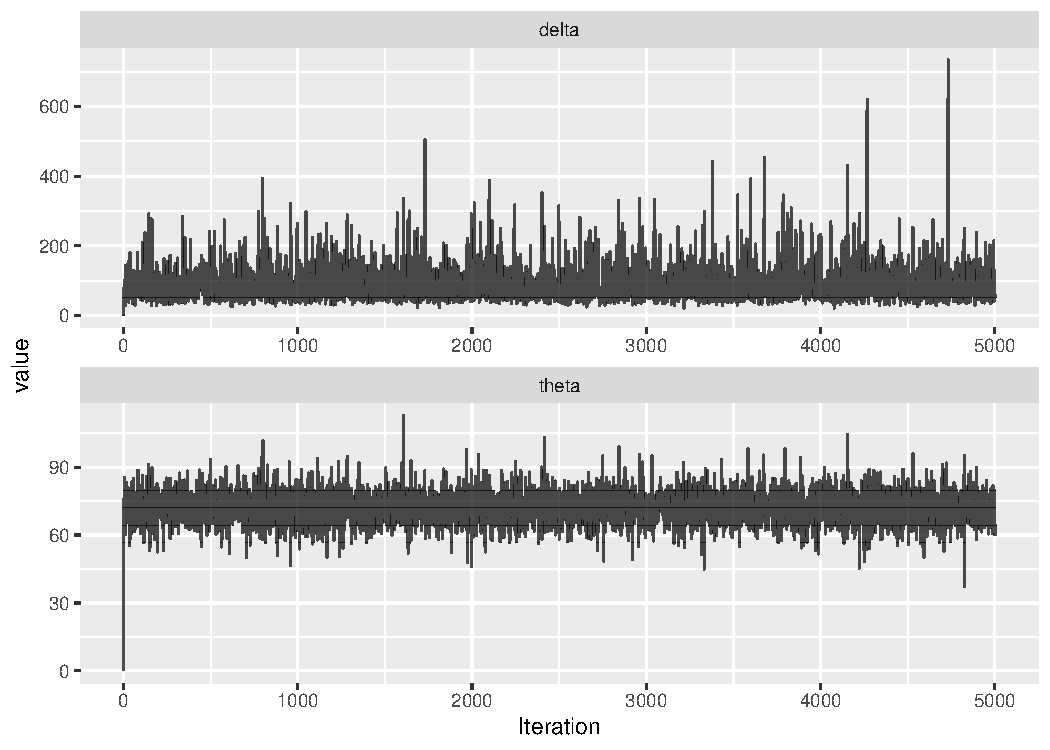
\includegraphics[width=0.8\linewidth]{Bayes_stat_hw3_files/figure-latex/unnamed-chunk-46-1} \end{center}

\begin{Shaded}
\begin{Highlighting}[]
\NormalTok{post\_3 }\SpecialCharTok{\%\textgreater{}\%}\NormalTok{ mcmc }\SpecialCharTok{\%\textgreater{}\%}\NormalTok{ ggs }\SpecialCharTok{\%\textgreater{}\%} \FunctionTok{ggs\_autocorrelation}\NormalTok{()}
\end{Highlighting}
\end{Shaded}

\begin{center}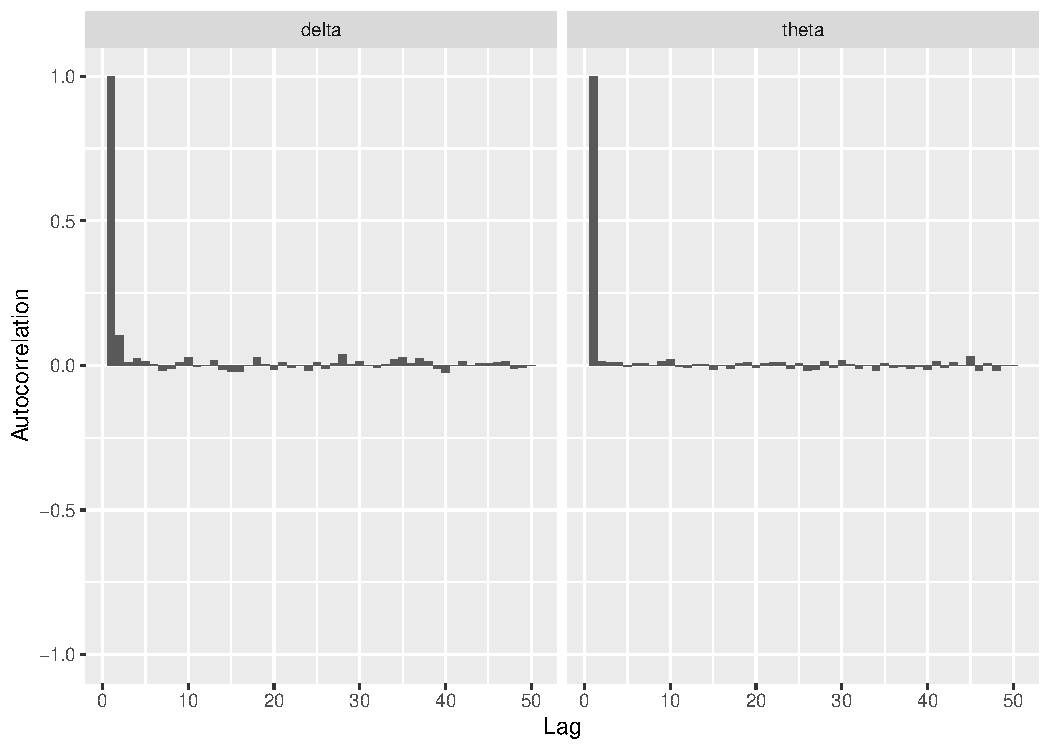
\includegraphics[width=0.8\linewidth]{Bayes_stat_hw3_files/figure-latex/unnamed-chunk-46-2} \end{center}

위와 같이 사후표본을 구한 결과, 마르코프 체인이 수렴했다고 보기에는 약간
미묘한 결과를 얻었다. prior 정보를 위와 같이 조정한 것은, 사전 정보를
정확히 조정할 근거가 없어 자료의 정보를 사용하되 nu0를 줄여 그 정보가
미치는 영향을 최대한 줄인 것이다. 충분히 수렴할 때까지 표본을 늘려
보았다.

\begin{Shaded}
\begin{Highlighting}[]
\CommentTok{\#가능도}
\NormalTok{df }\OtherTok{\textless{}{-}} \FunctionTok{c}\NormalTok{(}\FloatTok{68.3}\NormalTok{, }\FloatTok{85.7}\NormalTok{, }\FloatTok{73.8}\NormalTok{, }\FloatTok{83.2}\NormalTok{, }\FloatTok{58.9}\NormalTok{, }\FloatTok{72.7}\NormalTok{, }\FloatTok{70.5}\NormalTok{, }\FloatTok{58.7}\NormalTok{, }\FloatTok{74.1}\NormalTok{, }\FloatTok{75.0}\NormalTok{)}
\NormalTok{m }\OtherTok{\textless{}{-}} \DecValTok{50000}

\NormalTok{nu }\OtherTok{\textless{}{-}} \FunctionTok{length}\NormalTok{(df) }\CommentTok{\#prior의 정보 1}
\NormalTok{theta0 }\OtherTok{\textless{}{-}} \FunctionTok{mean}\NormalTok{(df) }\CommentTok{\#prior의 정보 2}
\NormalTok{nu0 }\OtherTok{\textless{}{-}} \DecValTok{1} \CommentTok{\#prior의 정보 3}
\NormalTok{s02 }\OtherTok{\textless{}{-}} \FunctionTok{var}\NormalTok{(df) }\CommentTok{\#prior의 정보 4}
\NormalTok{theta\_0 }\OtherTok{\textless{}{-}} \DecValTok{0}
\NormalTok{delta\_0 }\OtherTok{\textless{}{-}} \DecValTok{1}
\NormalTok{ksi\_0 }\OtherTok{\textless{}{-}} \DecValTok{0}
\NormalTok{po.theta }\OtherTok{=} \ConstantTok{NULL}
\NormalTok{po.delta }\OtherTok{=} \ConstantTok{NULL}
\NormalTok{po.ksi }\OtherTok{=} \ConstantTok{NULL}
\NormalTok{po.theta }\OtherTok{\textless{}{-}} \FunctionTok{c}\NormalTok{(po.theta, theta\_0)}
\NormalTok{po.delta }\OtherTok{\textless{}{-}} \FunctionTok{c}\NormalTok{(po.delta, delta\_0)}
\NormalTok{po.ksi }\OtherTok{\textless{}{-}} \FunctionTok{c}\NormalTok{(po.ksi, ksi\_0)}

\FunctionTok{set.seed}\NormalTok{(}\DecValTok{42}\NormalTok{)}
\ControlFlowTok{for}\NormalTok{ (i }\ControlFlowTok{in} \DecValTok{1}\SpecialCharTok{:}\NormalTok{m) \{}
\NormalTok{  ksi\_prime }\OtherTok{\textless{}{-}} \FunctionTok{rgamma}\NormalTok{(}\DecValTok{1}\NormalTok{, (}\DecValTok{1}\SpecialCharTok{+}\NormalTok{nu)}\SpecialCharTok{/}\DecValTok{2}\NormalTok{, }\AttributeTok{rate =} \DecValTok{1} \SpecialCharTok{+}\NormalTok{ ((po.theta[i]}\SpecialCharTok{{-}}\NormalTok{theta0)}\SpecialCharTok{\^{}}\DecValTok{2}\NormalTok{) }\SpecialCharTok{/}\NormalTok{ (nu}\SpecialCharTok{*}\NormalTok{po.delta[i]))}
\NormalTok{  theta\_prime }\OtherTok{\textless{}{-}} \FunctionTok{rnorm}\NormalTok{(}\DecValTok{1}\NormalTok{, (nu}\SpecialCharTok{*}\FunctionTok{mean}\NormalTok{(df) }\SpecialCharTok{+} \DecValTok{2}\SpecialCharTok{*}\NormalTok{theta0}\SpecialCharTok{*}\NormalTok{ksi\_prime) }\SpecialCharTok{/}\NormalTok{ (nu}\SpecialCharTok{+}\DecValTok{2}\SpecialCharTok{*}\NormalTok{ksi\_prime), }\FunctionTok{sqrt}\NormalTok{((nu}\SpecialCharTok{*}\NormalTok{po.delta[i]) }\SpecialCharTok{/}\NormalTok{ (nu}\SpecialCharTok{+}\DecValTok{2}\SpecialCharTok{*}\NormalTok{ksi\_prime)))}
\NormalTok{  delta\_rate }\OtherTok{=}\NormalTok{ (((nu }\SpecialCharTok{+} \DecValTok{2}\SpecialCharTok{*}\NormalTok{ksi\_prime)}\SpecialCharTok{*}\NormalTok{((theta\_prime }\SpecialCharTok{{-}}\NormalTok{ (nu}\SpecialCharTok{*}\FunctionTok{mean}\NormalTok{(df) }\SpecialCharTok{+} \DecValTok{2}\SpecialCharTok{*}\NormalTok{ksi\_prime}\SpecialCharTok{*}\NormalTok{theta0) }\SpecialCharTok{/}\NormalTok{ (nu }\SpecialCharTok{+} \DecValTok{2}\SpecialCharTok{*}\NormalTok{ksi\_prime))}\SpecialCharTok{\^{}}\DecValTok{2}\NormalTok{))}\SpecialCharTok{/}\NormalTok{(}\DecValTok{2}\SpecialCharTok{*}\NormalTok{nu))}\SpecialCharTok{+}\NormalTok{(}\DecValTok{1}\SpecialCharTok{/}\DecValTok{2}\NormalTok{)}\SpecialCharTok{*}\NormalTok{(nu0}\SpecialCharTok{*}\NormalTok{s02}\SpecialCharTok{+}\NormalTok{(}\FunctionTok{length}\NormalTok{(df)}\SpecialCharTok{{-}}\DecValTok{1}\NormalTok{)}\SpecialCharTok{*}\FunctionTok{var}\NormalTok{(df)}\SpecialCharTok{+}\NormalTok{(}\DecValTok{2}\SpecialCharTok{*}\NormalTok{ksi\_prime}\SpecialCharTok{*}\NormalTok{(}\FunctionTok{mean}\NormalTok{(df)}\SpecialCharTok{{-}}\NormalTok{theta0)}\SpecialCharTok{\^{}}\DecValTok{2}\NormalTok{)}\SpecialCharTok{/}\NormalTok{(nu}\SpecialCharTok{+}\DecValTok{2}\SpecialCharTok{*}\NormalTok{ksi\_prime))}
\NormalTok{  delta\_prime }\OtherTok{\textless{}{-}} \FunctionTok{rinvgamma}\NormalTok{(}\DecValTok{1}\NormalTok{, (nu0 }\SpecialCharTok{+} \FunctionTok{length}\NormalTok{(df) }\SpecialCharTok{+} \DecValTok{1}\NormalTok{)}\SpecialCharTok{/}\DecValTok{2}\NormalTok{, }\AttributeTok{rate =}\NormalTok{ delta\_rate)}
\NormalTok{  po.theta }\OtherTok{\textless{}{-}} \FunctionTok{c}\NormalTok{(po.theta, theta\_prime)}
\NormalTok{  po.delta }\OtherTok{\textless{}{-}} \FunctionTok{c}\NormalTok{(po.delta, delta\_prime)}
\NormalTok{  po.ksi }\OtherTok{\textless{}{-}} \FunctionTok{c}\NormalTok{(po.ksi, ksi\_prime)}
\NormalTok{\}}

\NormalTok{post\_4 }\OtherTok{\textless{}{-}} \FunctionTok{data.frame}\NormalTok{(}\AttributeTok{theta =}\NormalTok{ po.theta, }\AttributeTok{delta =}\NormalTok{ po.delta)}
\end{Highlighting}
\end{Shaded}

\begin{Shaded}
\begin{Highlighting}[]
\NormalTok{post\_4 }\SpecialCharTok{\%\textgreater{}\%}\NormalTok{ mcmc }\SpecialCharTok{\%\textgreater{}\%}\NormalTok{ ggs }\SpecialCharTok{\%\textgreater{}\%} \FunctionTok{ggs\_traceplot}\NormalTok{()}
\end{Highlighting}
\end{Shaded}

\begin{center}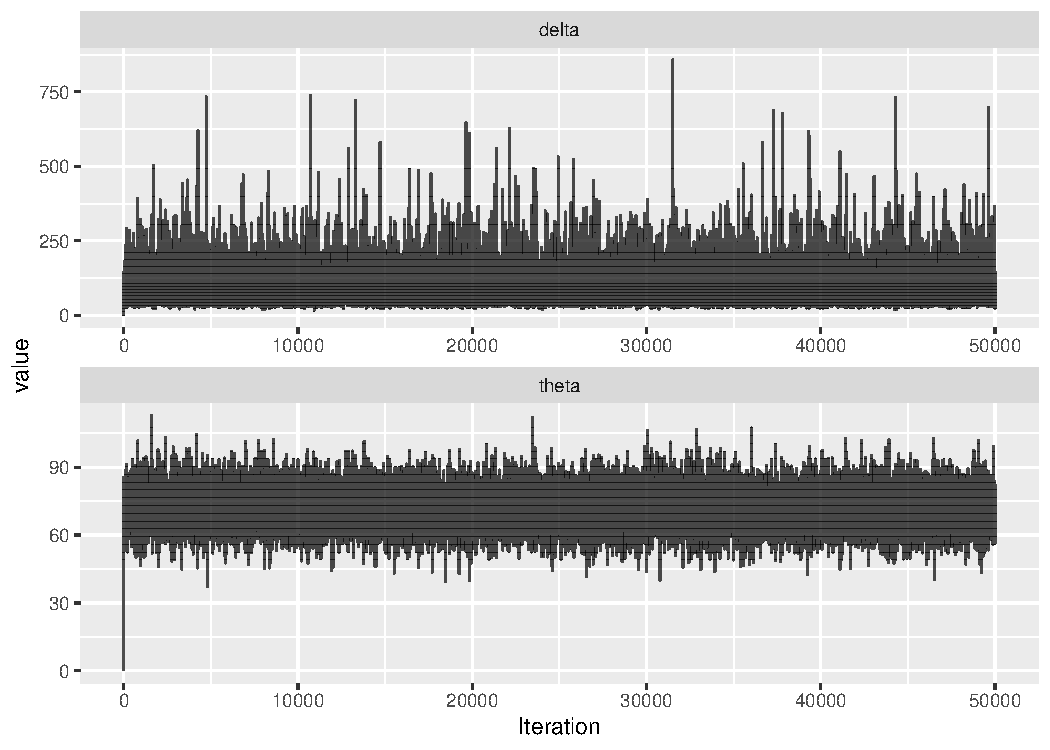
\includegraphics[width=0.8\linewidth]{Bayes_stat_hw3_files/figure-latex/unnamed-chunk-48-1} \end{center}

\begin{Shaded}
\begin{Highlighting}[]
\NormalTok{post\_4 }\SpecialCharTok{\%\textgreater{}\%}\NormalTok{ mcmc }\SpecialCharTok{\%\textgreater{}\%}\NormalTok{ ggs }\SpecialCharTok{\%\textgreater{}\%} \FunctionTok{ggs\_autocorrelation}\NormalTok{()}
\end{Highlighting}
\end{Shaded}

\begin{center}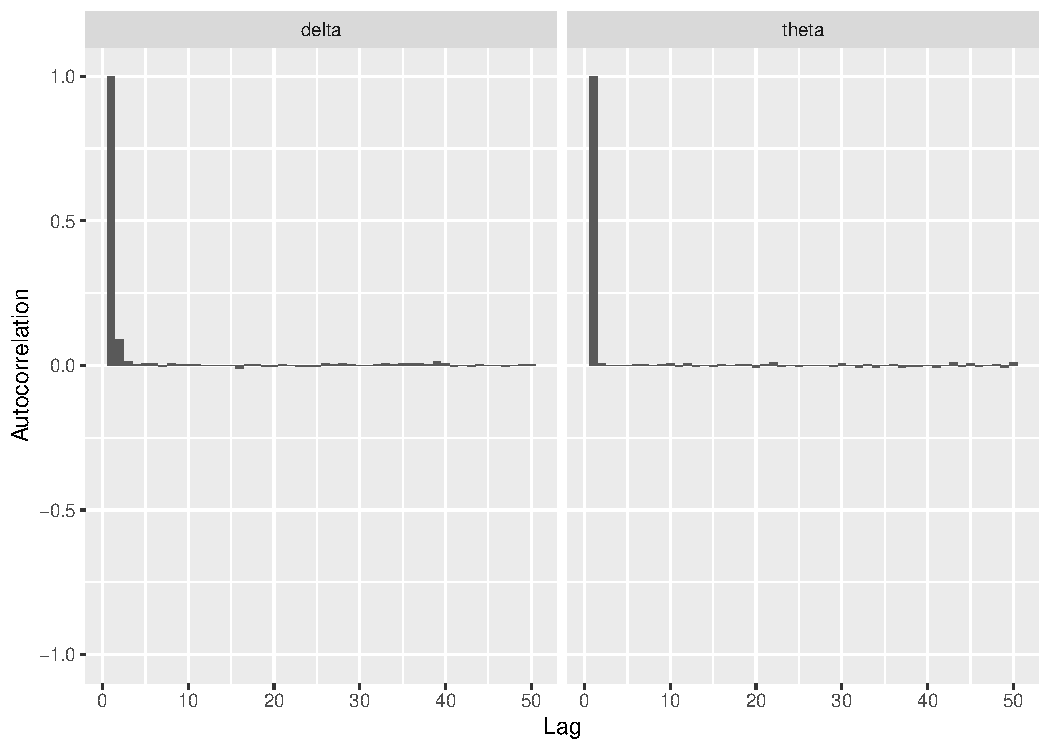
\includegraphics[width=0.8\linewidth]{Bayes_stat_hw3_files/figure-latex/unnamed-chunk-48-2} \end{center}

m = 50000 수준에서는 충분히 수렴했다고 판단할 수 있다. 이를 사용한다.

\subsection{(e)}\label{e}

\begin{Shaded}
\begin{Highlighting}[]
\NormalTok{post\_4 }\SpecialCharTok{\%\textgreater{}\%}\NormalTok{ mcmc }\SpecialCharTok{\%\textgreater{}\%}\NormalTok{ ggs }\SpecialCharTok{\%\textgreater{}\%} \FunctionTok{ggs\_histogram}\NormalTok{()}
\end{Highlighting}
\end{Shaded}

\begin{center}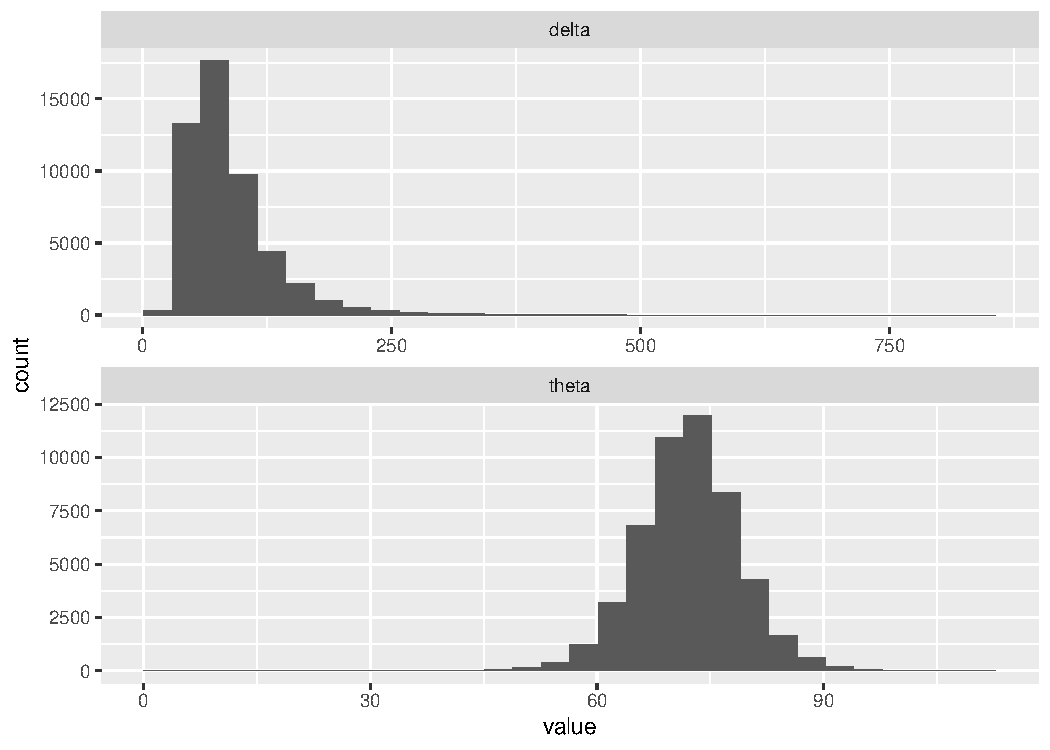
\includegraphics[width=0.8\linewidth]{Bayes_stat_hw3_files/figure-latex/unnamed-chunk-49-1} \end{center}

\begin{Shaded}
\begin{Highlighting}[]
\NormalTok{post\_4 }\SpecialCharTok{\%\textgreater{}\%}\NormalTok{ mcmc }\SpecialCharTok{\%\textgreater{}\%}\NormalTok{ ggs }\SpecialCharTok{\%\textgreater{}\%} \FunctionTok{ggs\_density}\NormalTok{()}
\end{Highlighting}
\end{Shaded}

\begin{center}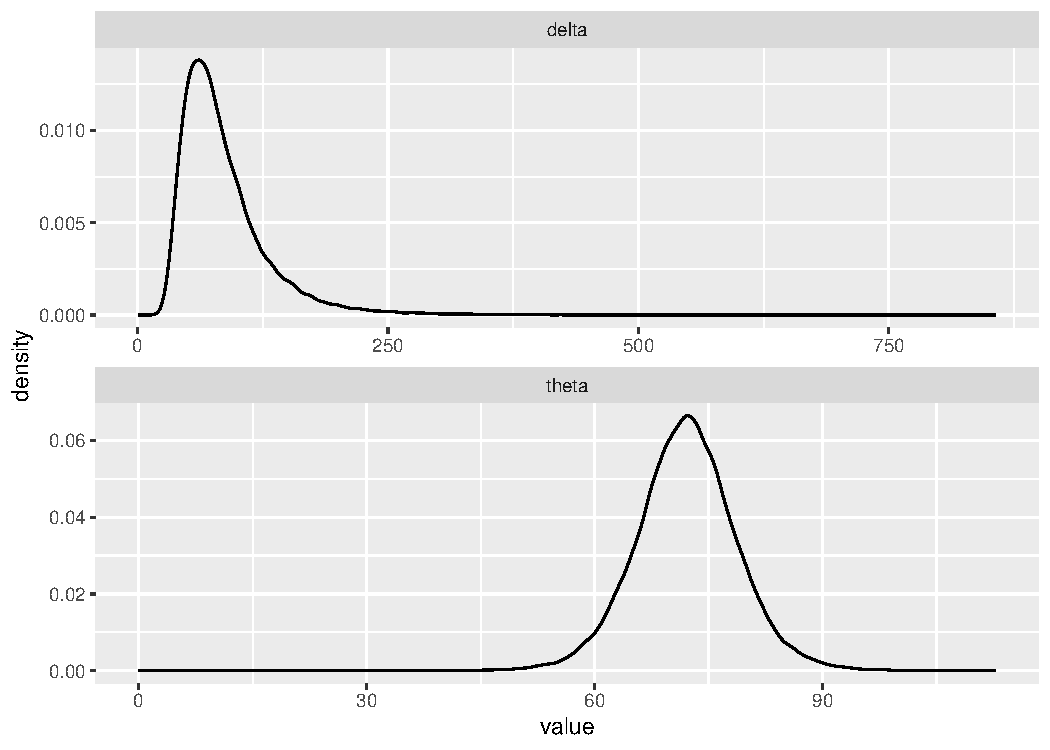
\includegraphics[width=0.8\linewidth]{Bayes_stat_hw3_files/figure-latex/unnamed-chunk-49-2} \end{center}

사후표본의 히스토그램과 밀도함수 그림은 다음과 같다.

\subsection{(f)}\label{f}

\begin{Shaded}
\begin{Highlighting}[]
\NormalTok{post\_4 }\SpecialCharTok{\%\textgreater{}\%}\NormalTok{ mcmc }\SpecialCharTok{\%\textgreater{}\%}\NormalTok{ summary}
\end{Highlighting}
\end{Shaded}

\begin{verbatim}
## 
## Iterations = 1:50001
## Thinning interval = 1 
## Number of chains = 1 
## Sample size per chain = 50001 
## 
## 1. Empirical mean and standard deviation for each variable,
##    plus standard error of the mean:
## 
##        Mean     SD Naive SE Time-series SE
## theta 72.10  6.651  0.02974        0.02995
## delta 86.13 46.165  0.20646        0.22564
## 
## 2. Quantiles for each variable:
## 
##        2.5%   25%   50%    75%  97.5%
## theta 58.90 67.94 72.08  76.21  85.58
## delta 35.27 56.43 74.94 102.13 203.69
\end{verbatim}

theta의 사후평균 : 72.10 theta의 사후표준편차 : 6.651 theta의 95\% CI :
(58.90, 85.58)

sigma의 사후평균 : 9.280625 sigma의 사후표준편차 : 6.794483 sigma의 95\%
CI : (5.938855, 14.272)

\end{document}
